\documentclass[fleqn]{article}
\usepackage[utf8]{inputenc}
\usepackage{graphicx}
\usepackage{geometry}
\usepackage[fleqn]{amsmath}
\usepackage{tikz}
\usepackage{grffile}
\usepackage{hyperref}
\usepackage{epstopdf}
\usepackage{longtable}
\usepackage{subcaption}
\usepackage{capt-of}
\usepackage{tabu}

\graphicspath{{./pics}}
\newgeometry{left=3cm, top=2cm, bottom=2cm}
\newcommand{\noimage}{%
  \setlength{\fboxsep}{-\fboxrule}%
  \fbox{\phantom{\rule{150pt}{100pt}}}% Framed box
}
\newcommand{\myparagraph}[1]{\paragraph{#1}\mbox{}\\}

\title{EE6130 Machine Learning for Computer Vision\\ Assignment-2 \\(K-means, EM, Regression Algorithms))}
\author{Arulkumar S (CS15S023)}

\begin{document}
\setcounter{secnumdepth}{5}
\tracingall
\maketitle

\section{Image segmentation using K-Means clustering}

\subsection{segmentation of spectrum.png $(K=7)$}

\subsubsection{Mean values from centre-row}

The initial mean values are selected from pixels equally spaced in the horizontal direction in the centre row of
the image.\\\\
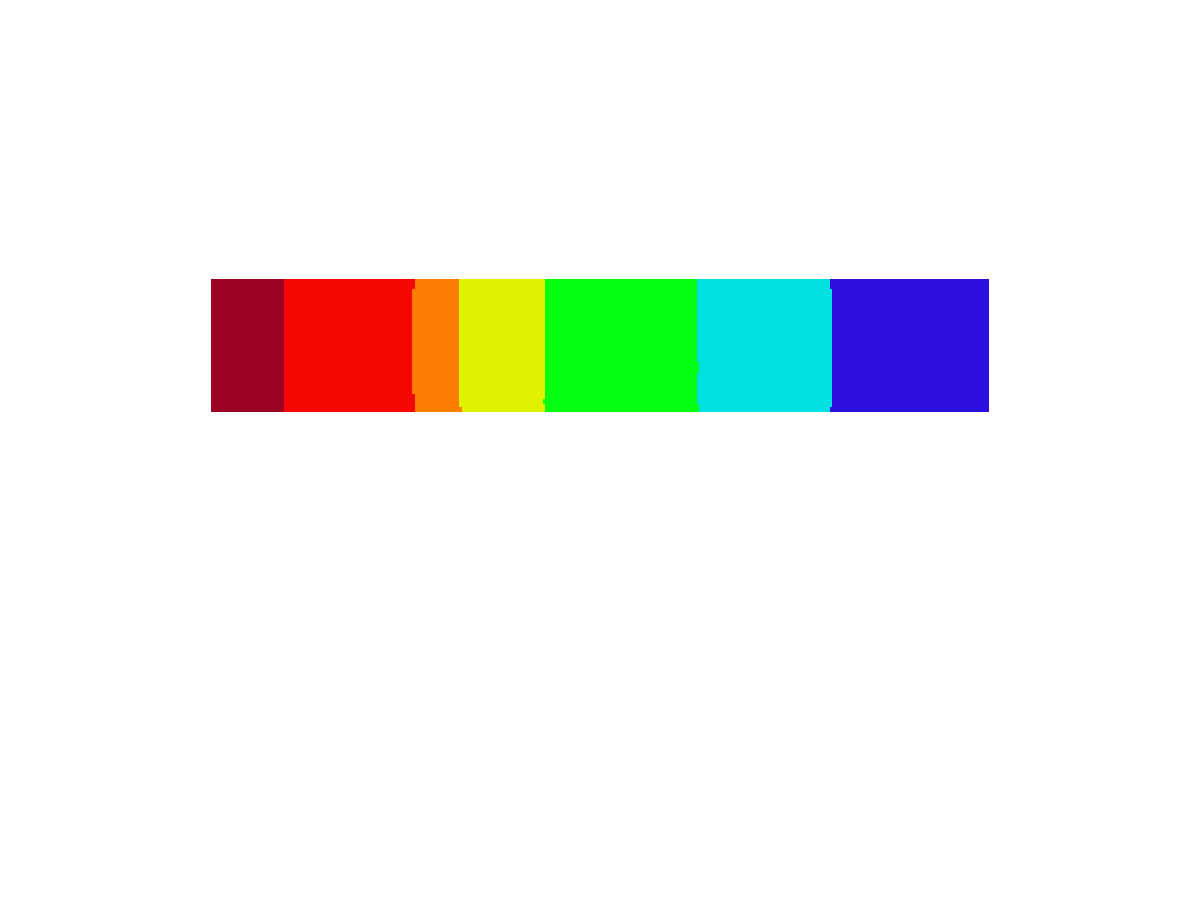
\includegraphics[scale=0.4]{./pics/task1and2/spectrum_k=7_equidistant/K=7_iteration_14_mid_equidistant_7_spectrum.png}\\ 
\begin{center}
  \begin{longtable}{ c | c }
	\multicolumn{1}{c}{iteration vs. cost} & 
	\multicolumn{1}{c}{iteration vs. cluster assignment changes}  \\
    \hline
    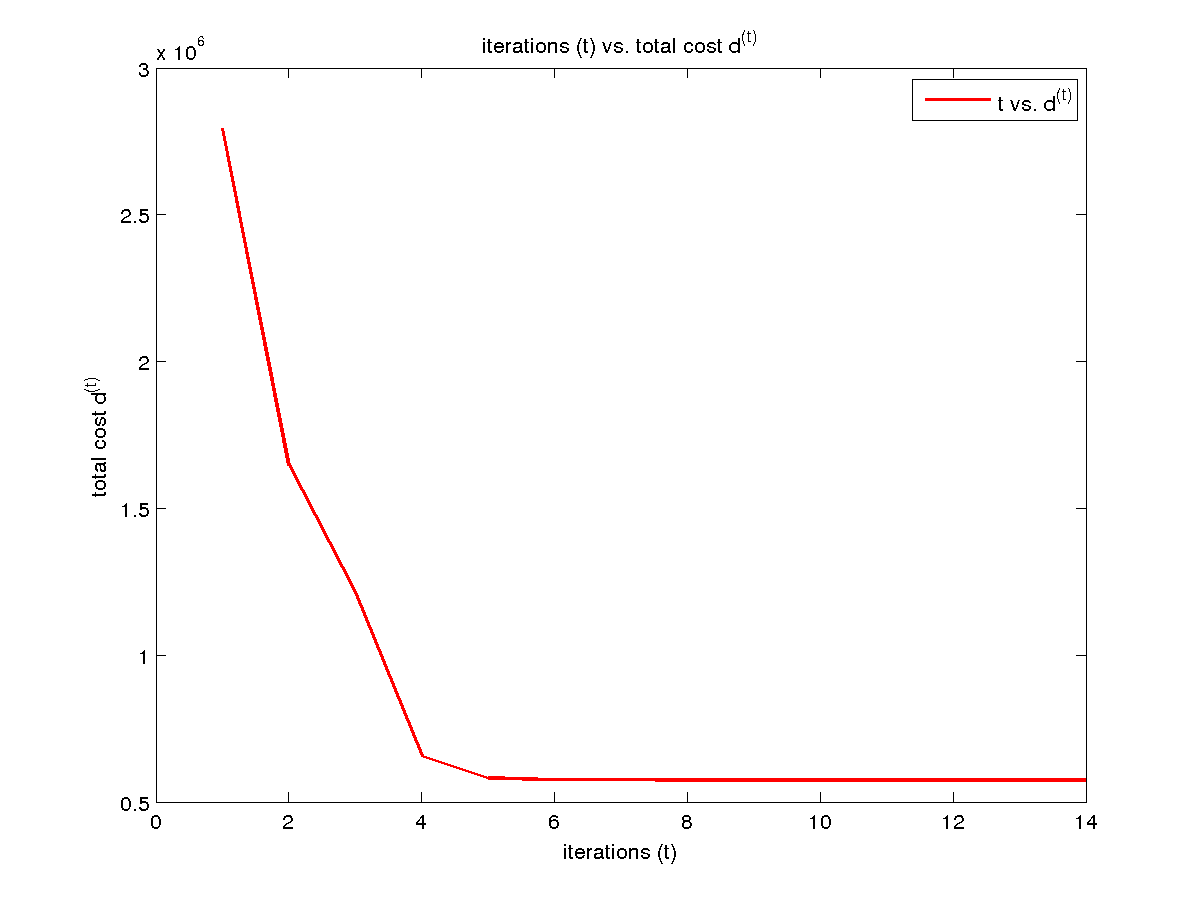
\includegraphics[scale=0.4]{./pics/task1and2/spectrum_k=7_equidistant/t_vs_d_mid_equidistant_7_spectrum.png}  & 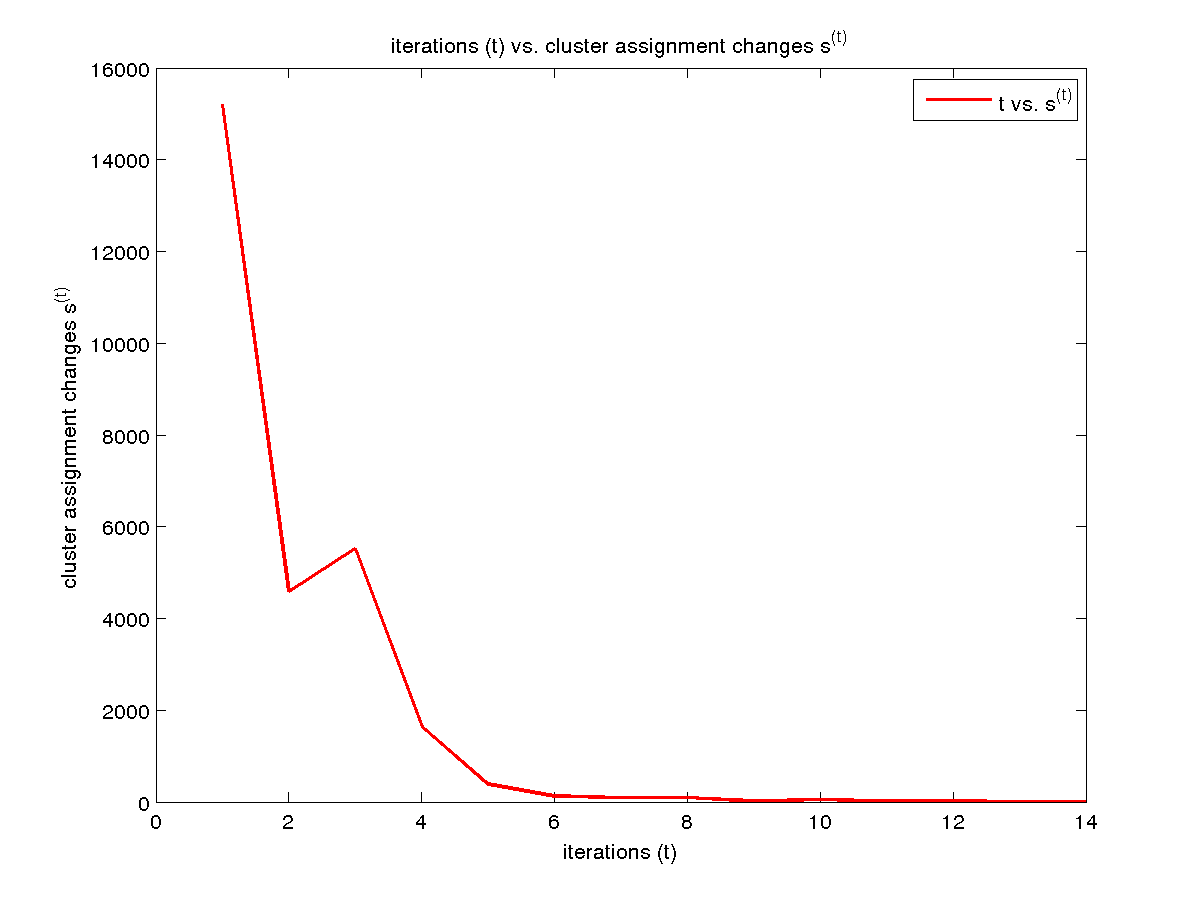
\includegraphics[scale=0.4]{./pics/task1and2/spectrum_k=7_equidistant/t_vs_s_mid_equidistant_7_spectrum.png} \\
    \hline
  \end{longtable}
\end{center}

\subsubsection{Random mean values}

Here, the mean values are chosen randomly from the available pixel values and K-means clustering is carried out until convergence.

\myparagraph{Random initialization-1}

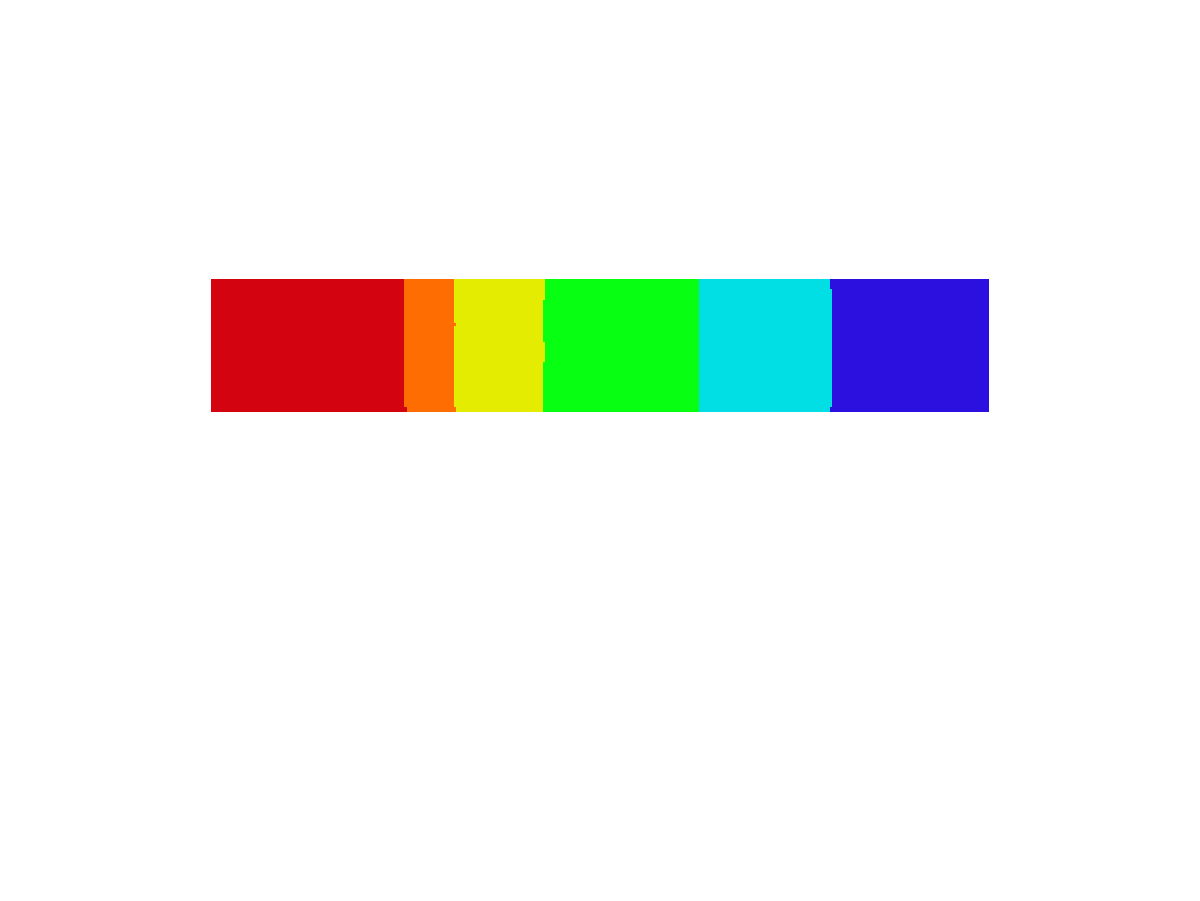
\includegraphics[scale=0.4]{./pics/task1and2/spectrum_k=7_random1/K=7_iteration_10_random_7_spectrum.png}\\ 
\begin{center}
  \begin{longtable}{ c | c }
	\multicolumn{1}{c}{iteration vs. cost} & 
	\multicolumn{1}{c}{iteration vs. cluster assignment changes}  \\
    \hline
    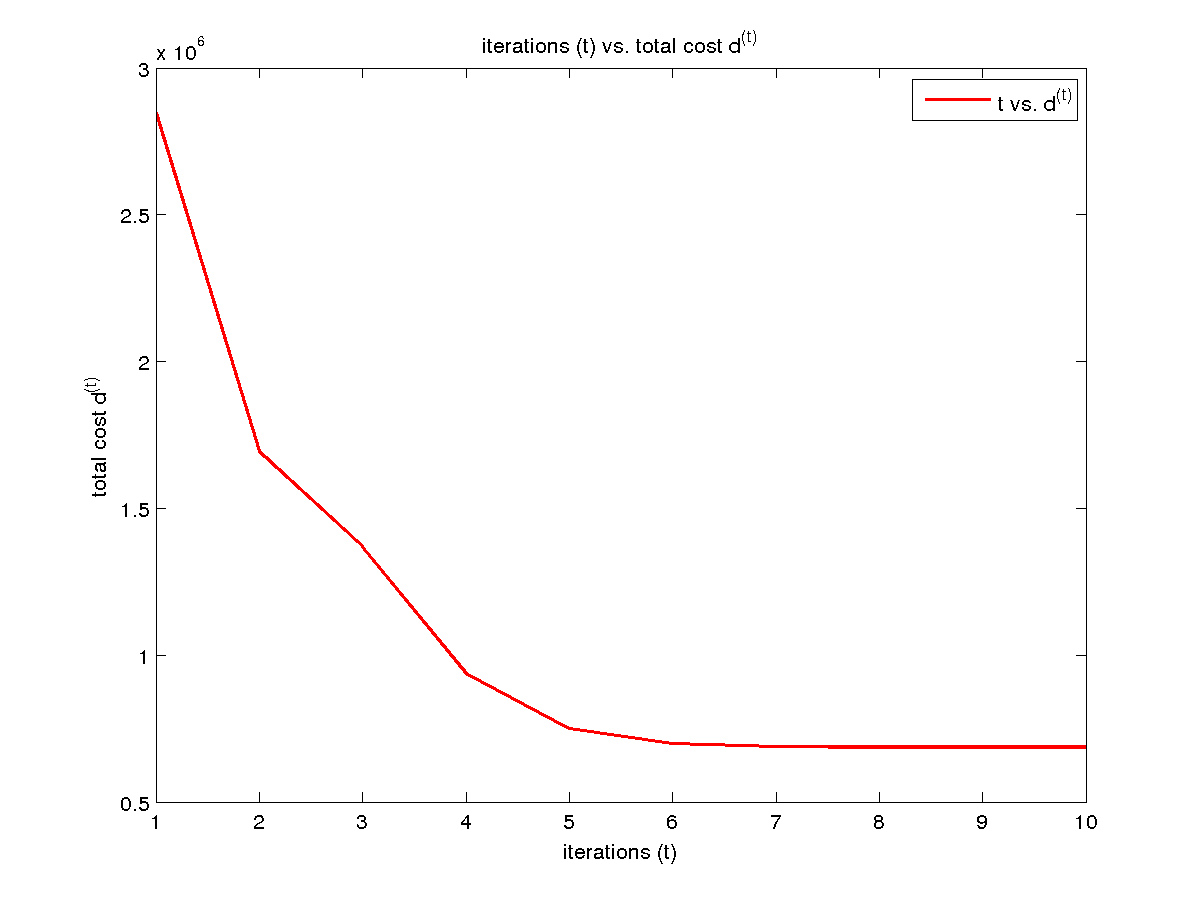
\includegraphics[scale=0.4]{./pics/task1and2/spectrum_k=7_random1/t_vs_d_random_7_spectrum.png}  & 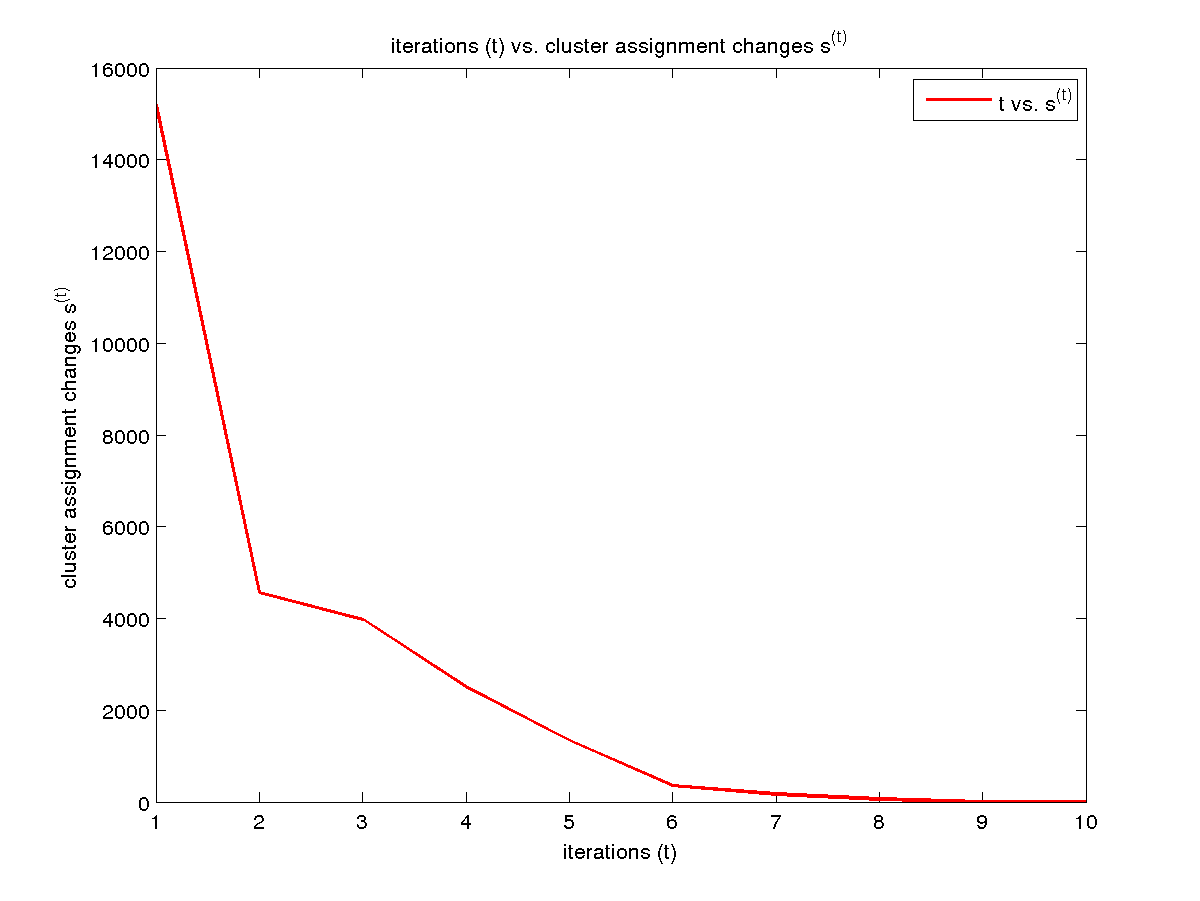
\includegraphics[scale=0.4]{./pics/task1and2/spectrum_k=7_random1/t_vs_s_random_7_spectrum.png} \\
    \hline
  \end{longtable}
\end{center}

\myparagraph{Random initialization-2}

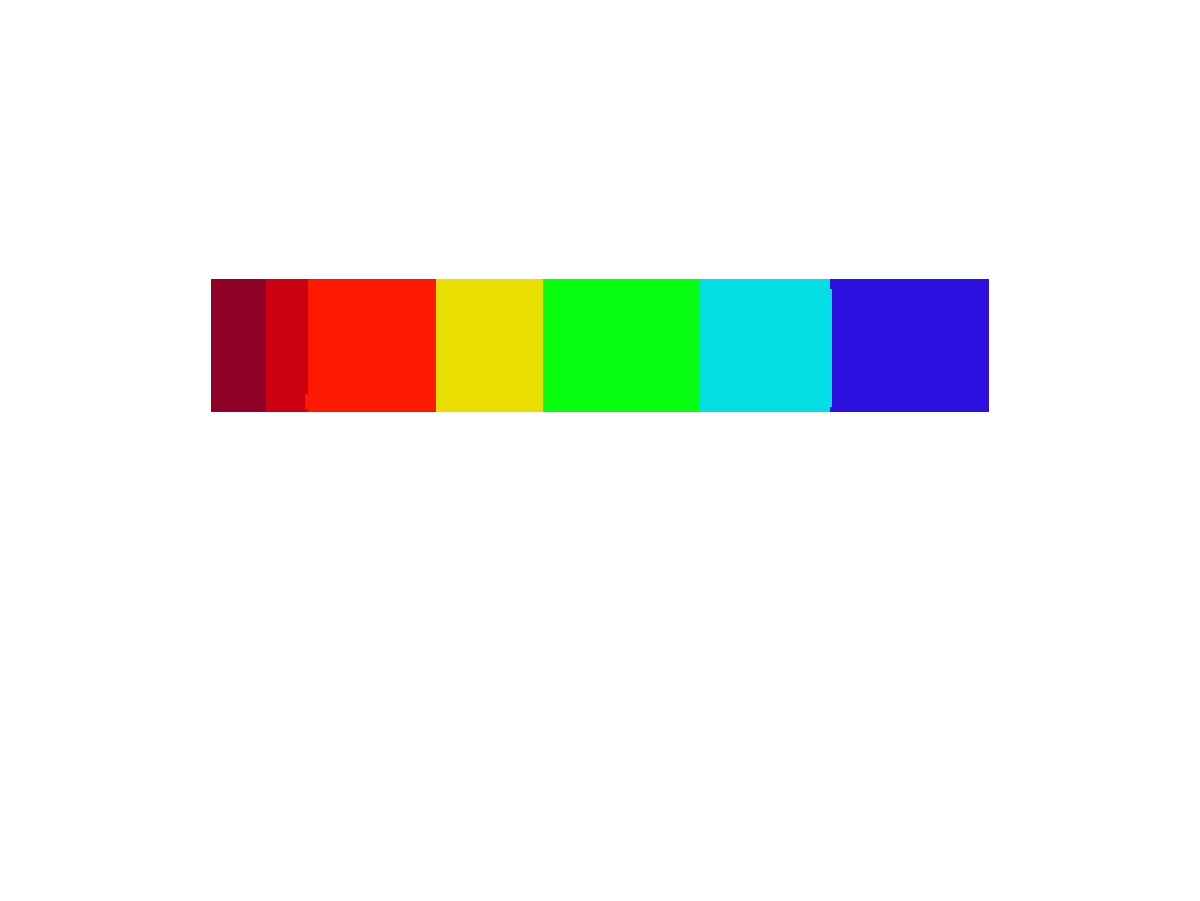
\includegraphics[scale=0.4]{./pics/task1and2/spectrum_k=7_random2/K=7_iteration_19_random_7_spectrum.png}\\ 
\begin{center}
  \begin{longtable}{ c | c }
	\multicolumn{1}{c}{iteration vs. cost} & 
	\multicolumn{1}{c}{iteration vs. cluster assignment changes}  \\
    \hline
    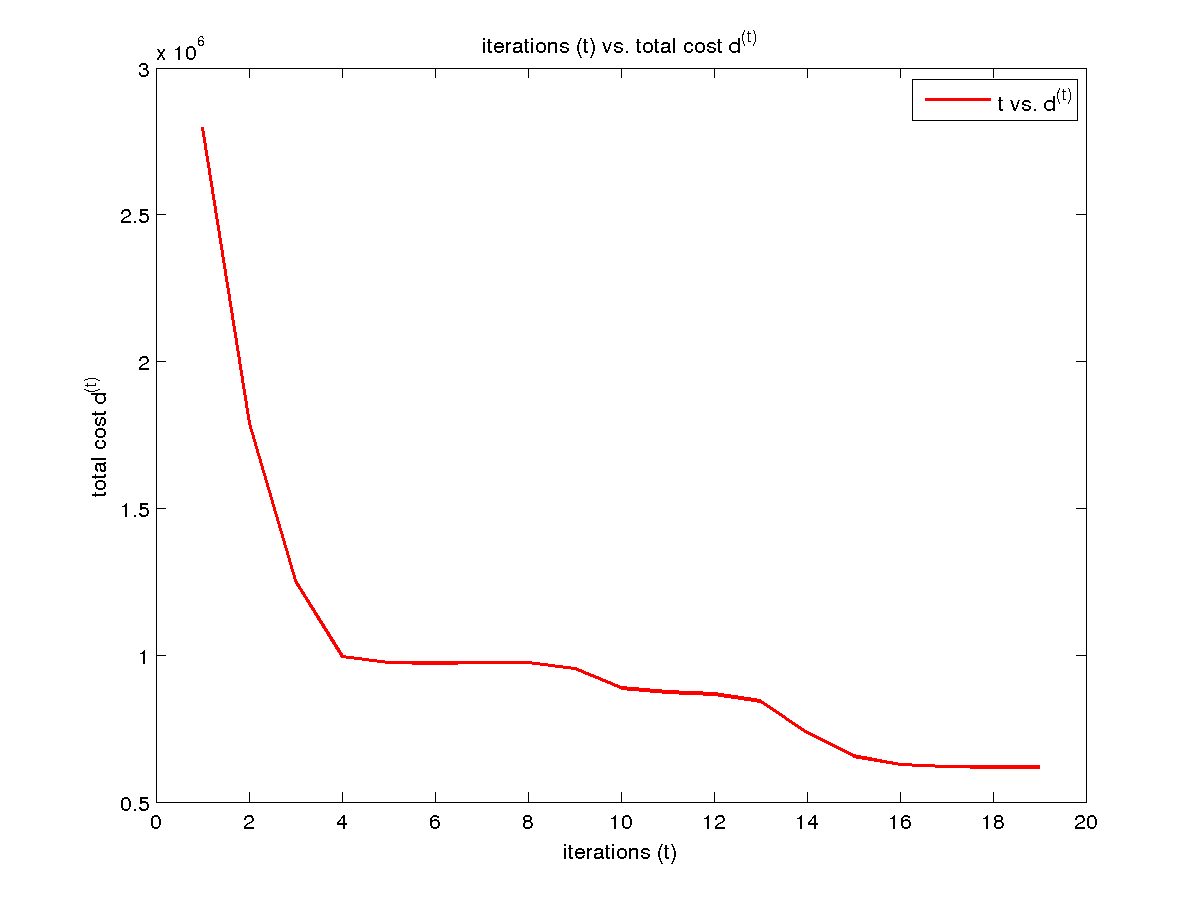
\includegraphics[scale=0.4]{./pics/task1and2/spectrum_k=7_random2/t_vs_d_random_7_spectrum.png}  & 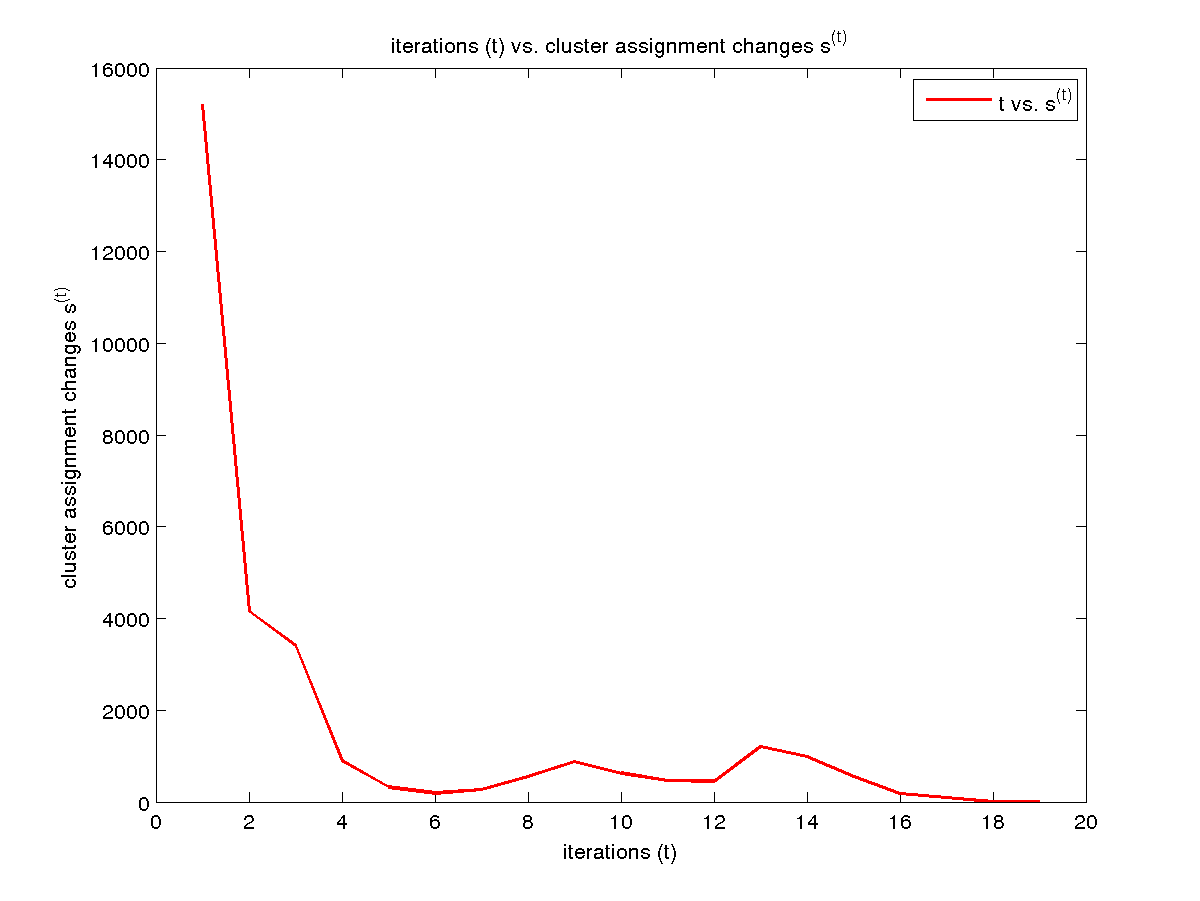
\includegraphics[scale=0.4]{./pics/task1and2/spectrum_k=7_random2/t_vs_s_random_7_spectrum.png} \\
    \hline
  \end{longtable}
\end{center}

As we can see in the segmented images from K-means clustering (randomly initialized means), 
\begin{itemize}
  \item K-means clustering is able to find local minimum of cost function depending on the initialization of means
  \item Comparing ``Random initialization-1'' with ``Random initialization-2'', it can be inferred that the segmented images are different \& it is not guaranteed that the segmented images will be same.
  \item In the K-means clustering process with the means initialized from centre row (equi-distant), since the means are initialized to cover the major colors in the image, the clustering result is always the same. 
\end{itemize}
\subsection{segmentation of rio.png}

\subsubsection{number of clusters = 2}

\begin{center}
  \begin{longtable}{ c | c }
	\multicolumn{1}{c}{} & 
	\multicolumn{1}{c}{}  \\
	
\includegraphics[scale=0.4]{./pics/task1and2/rio_k=2_random/K=2_iteration_1_random_2_rio.png} & 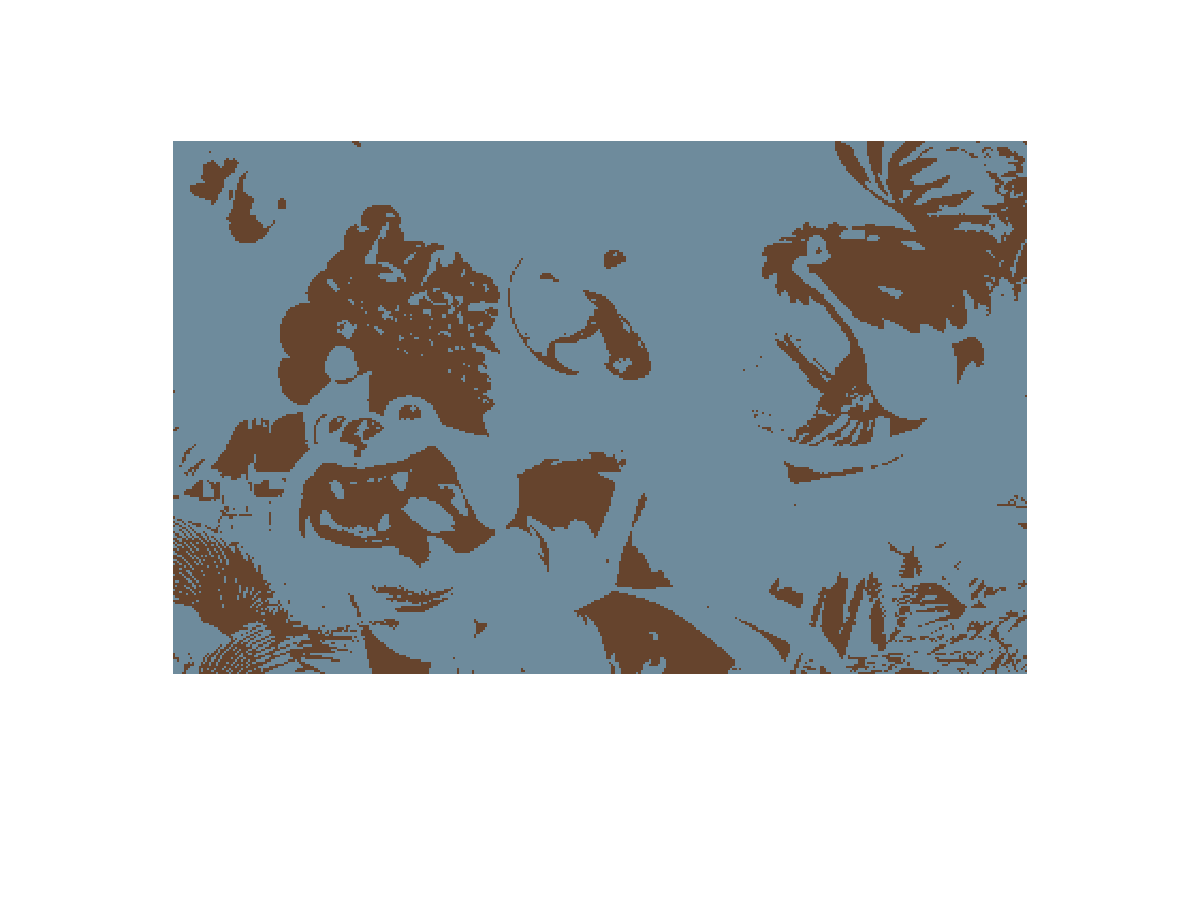
\includegraphics[scale=0.4]{./pics/task1and2/rio_k=2_random/K=2_iteration_2_random_2_rio.png} \\\hline
	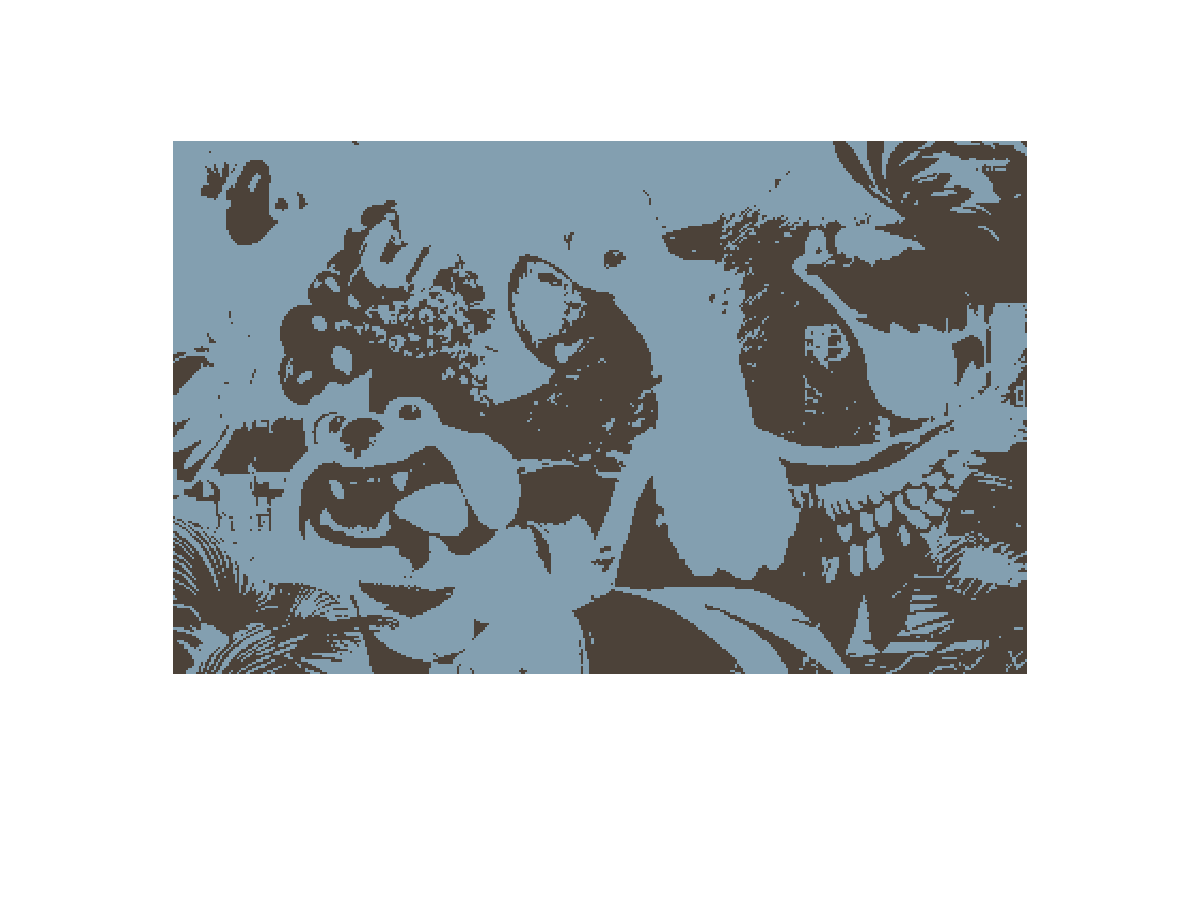
\includegraphics[scale=0.4]{./pics/task1and2/rio_k=2_random/K=2_iteration_3_random_2_rio.png} & 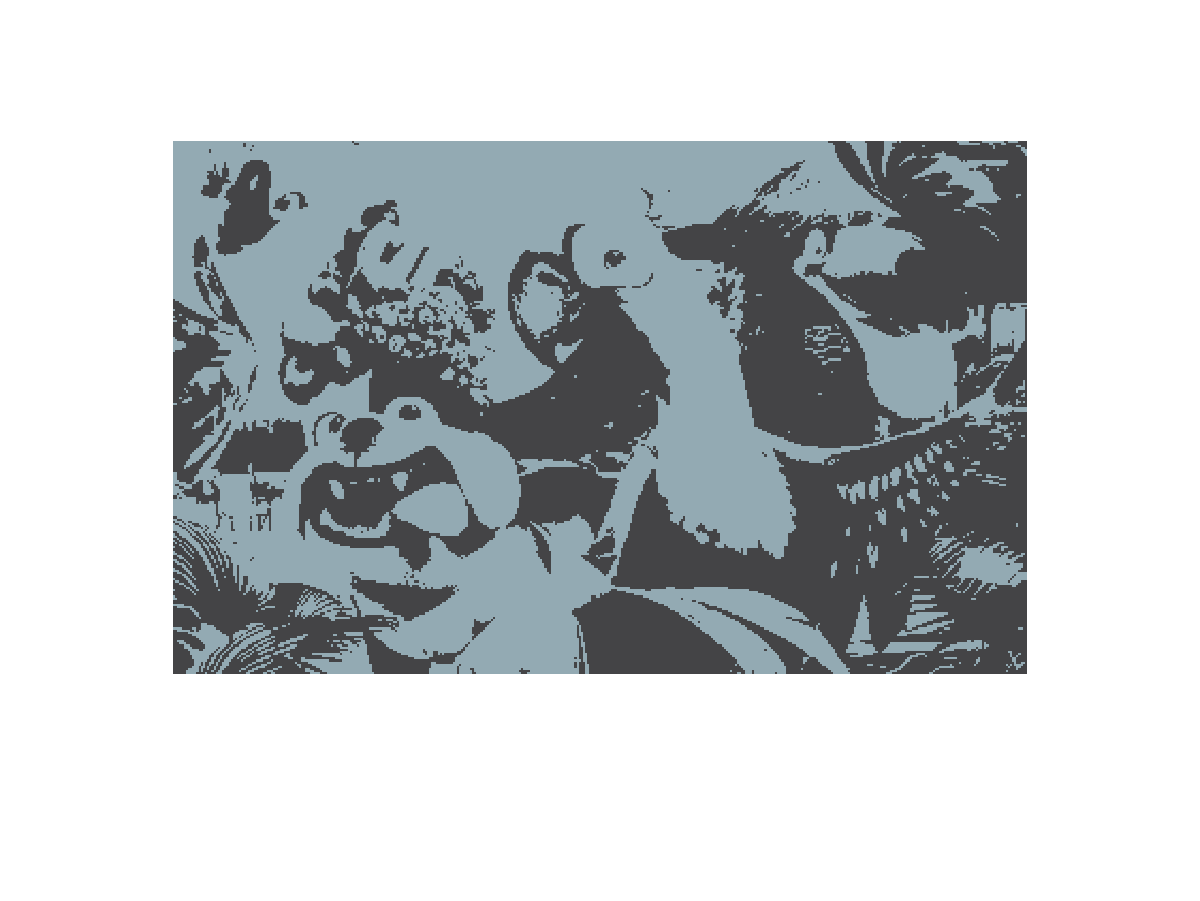
\includegraphics[scale=0.4]{./pics/task1and2/rio_k=2_random/K=2_iteration_4_random_2_rio.png} \\\hline
	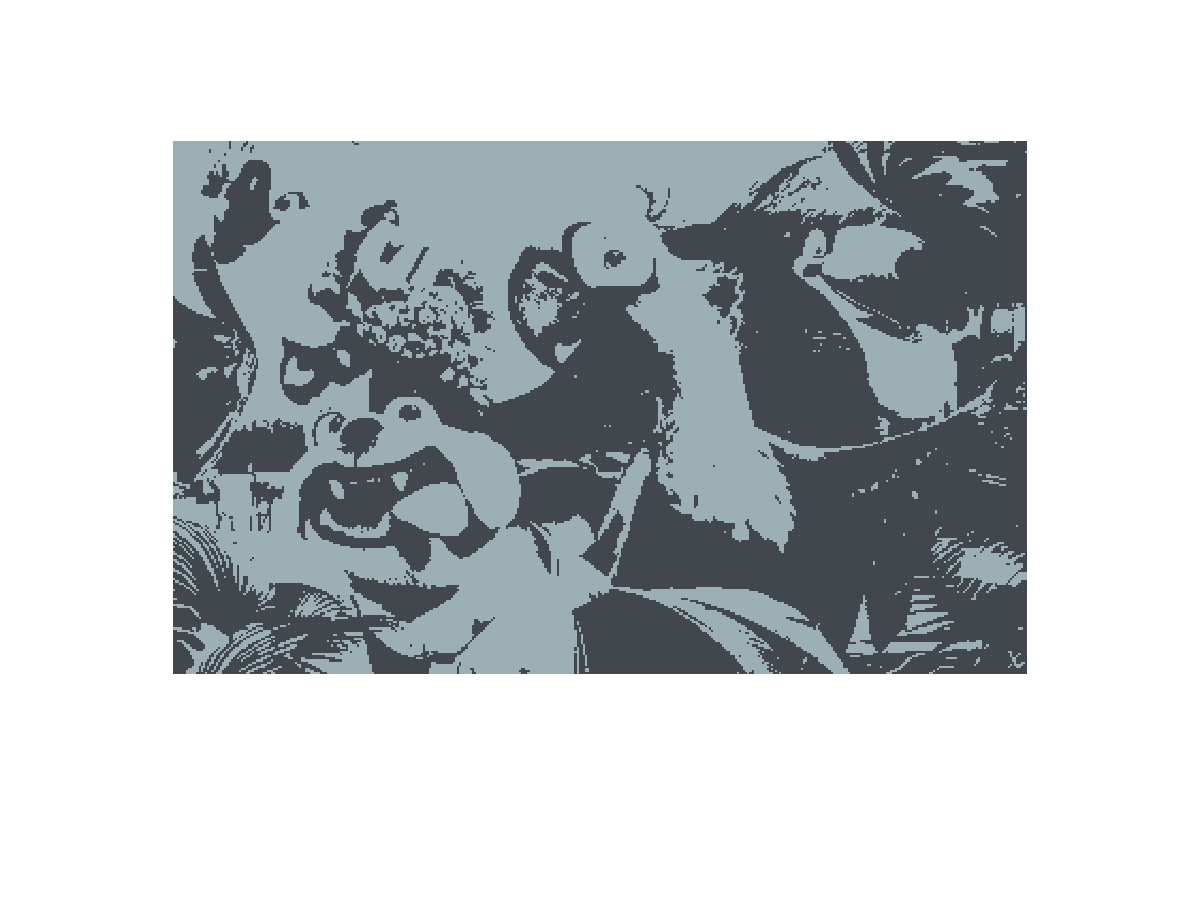
\includegraphics[scale=0.4]{./pics/task1and2/rio_k=2_random/K=2_iteration_5_random_2_rio.png} & 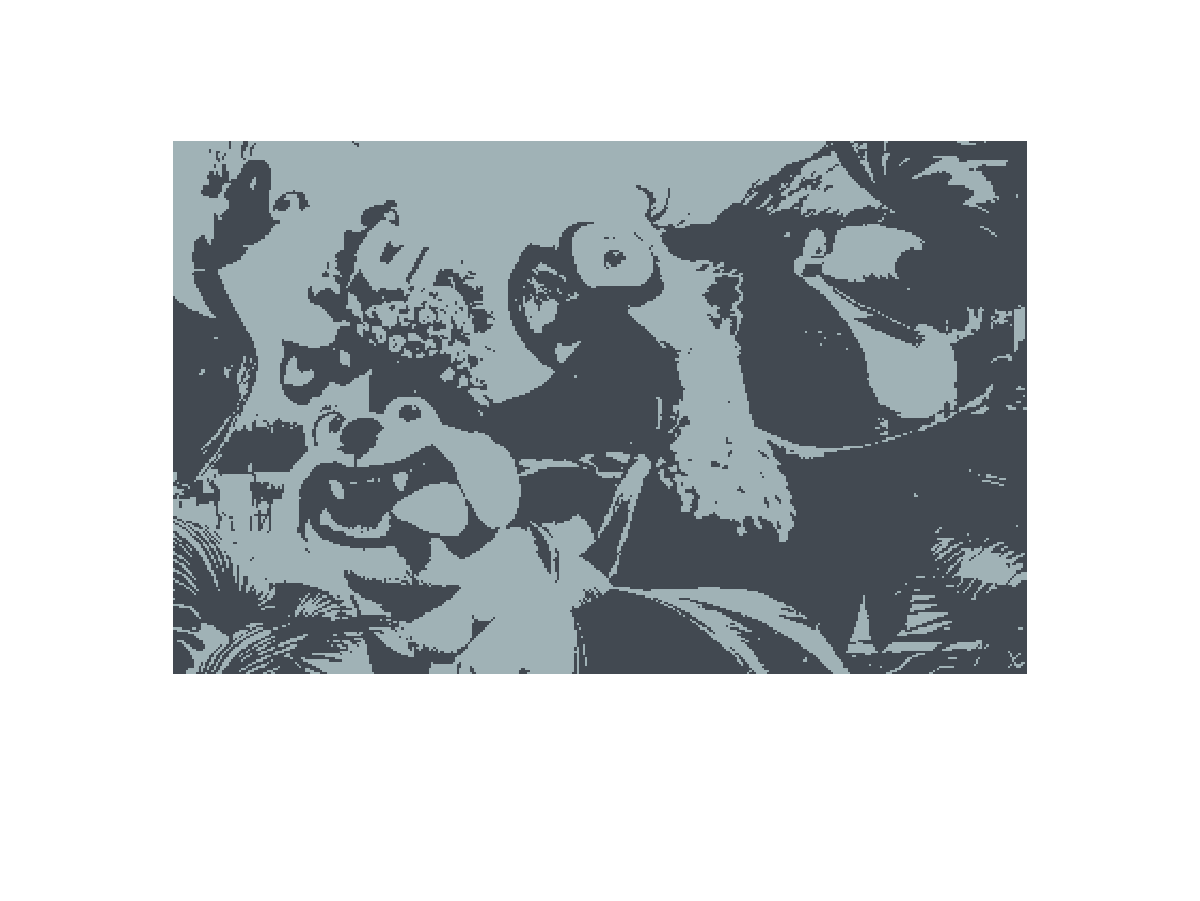
\includegraphics[scale=0.4]{./pics/task1and2/rio_k=2_random/K=2_iteration_6_random_2_rio.png} \\\hline
	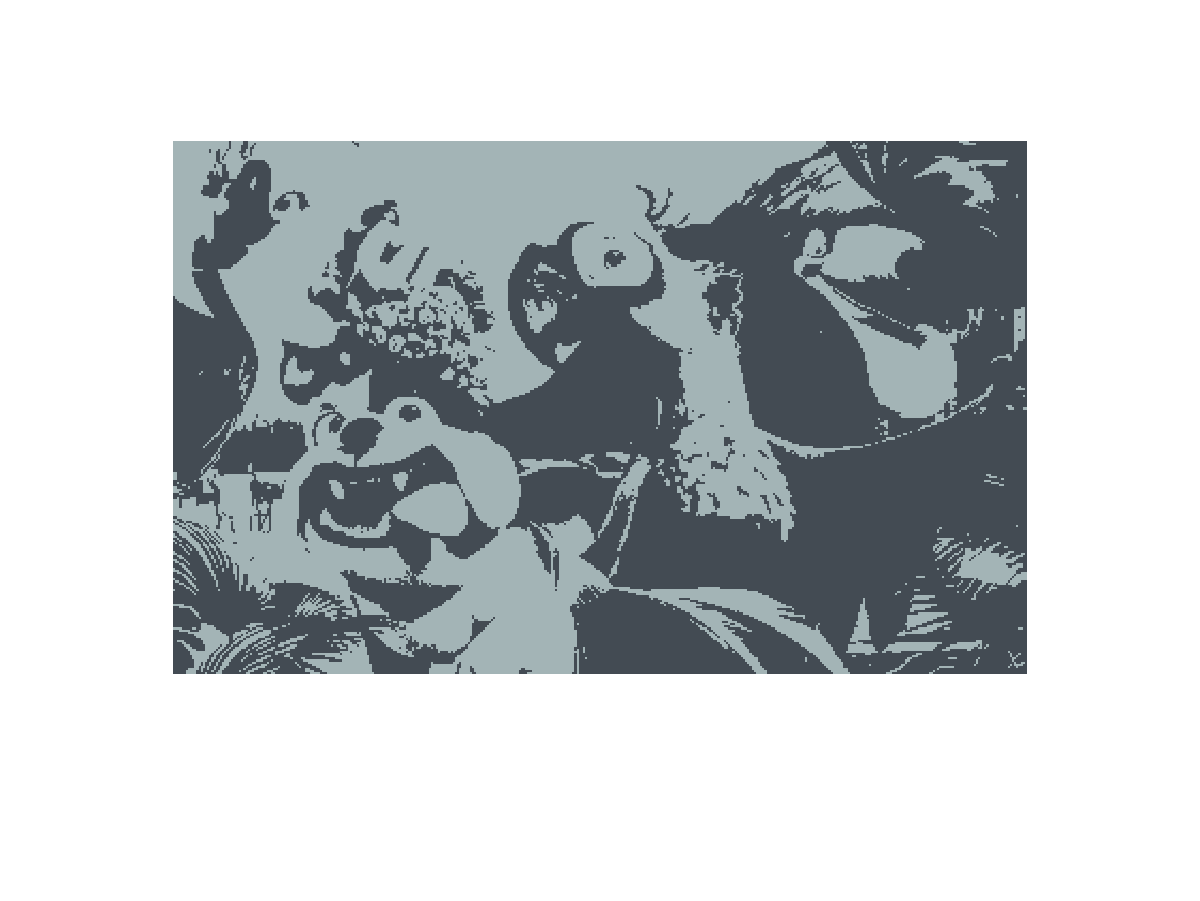
\includegraphics[scale=0.4]{./pics/task1and2/rio_k=2_random/K=2_iteration_7_random_2_rio.png} & 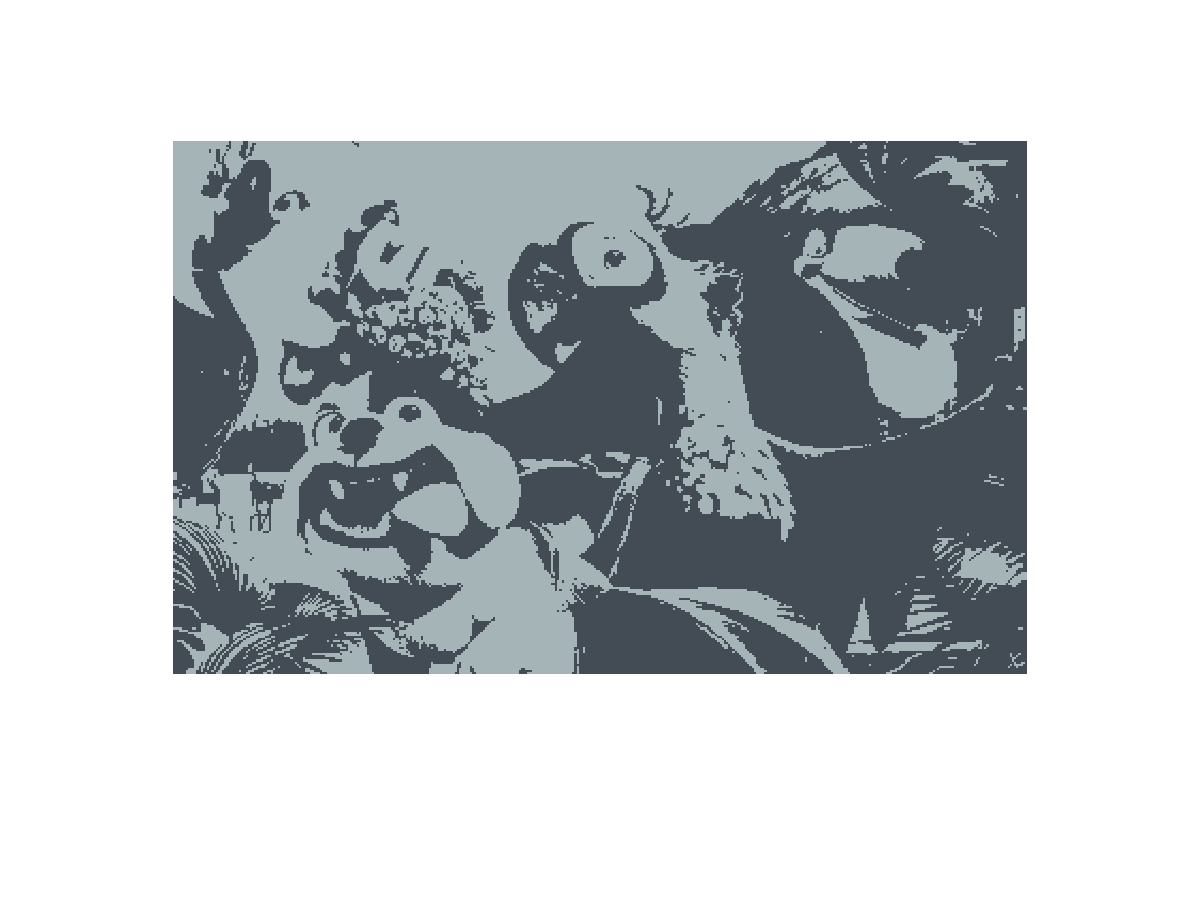
\includegraphics[scale=0.4]{./pics/task1and2/rio_k=2_random/K=2_iteration_8_random_2_rio.png} \\\hline
	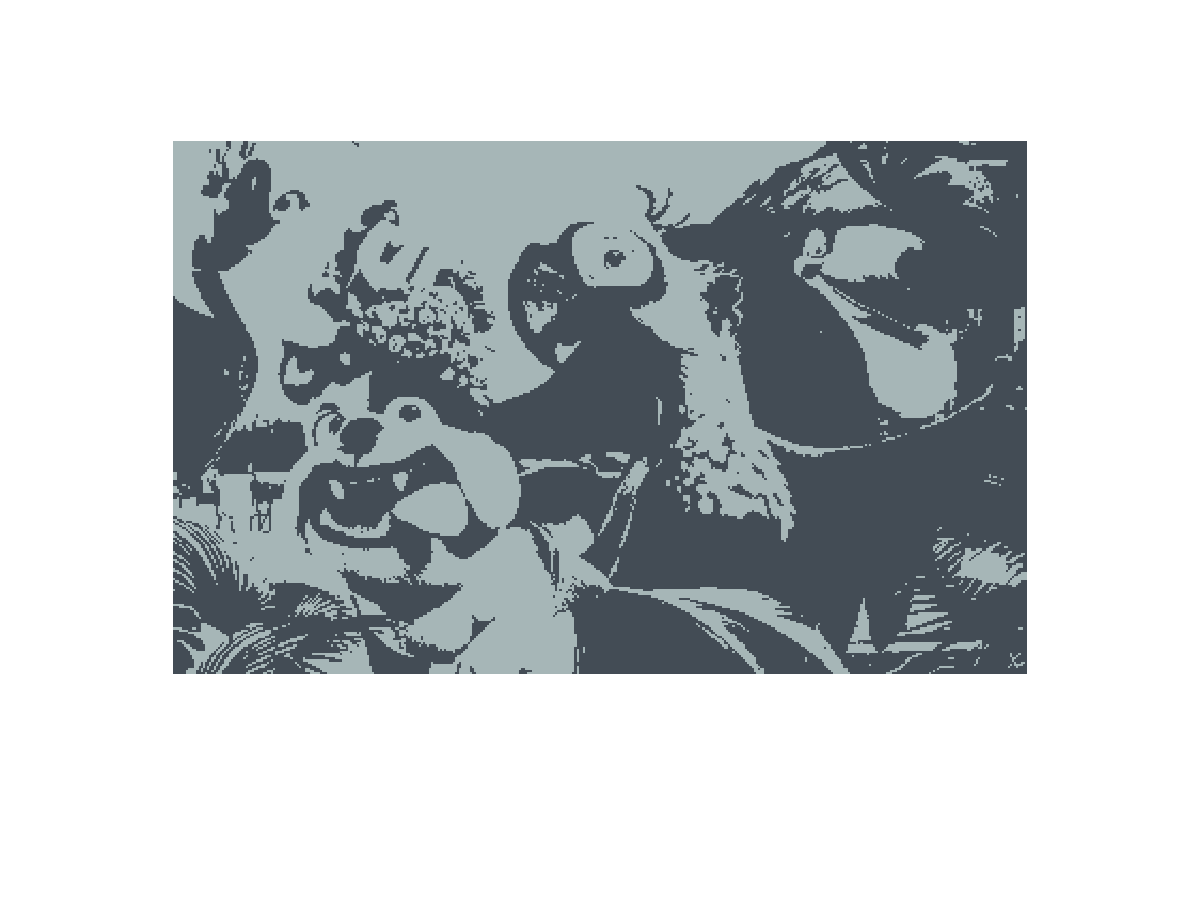
\includegraphics[scale=0.4]{./pics/task1and2/rio_k=2_random/K=2_iteration_9_random_2_rio.png} & 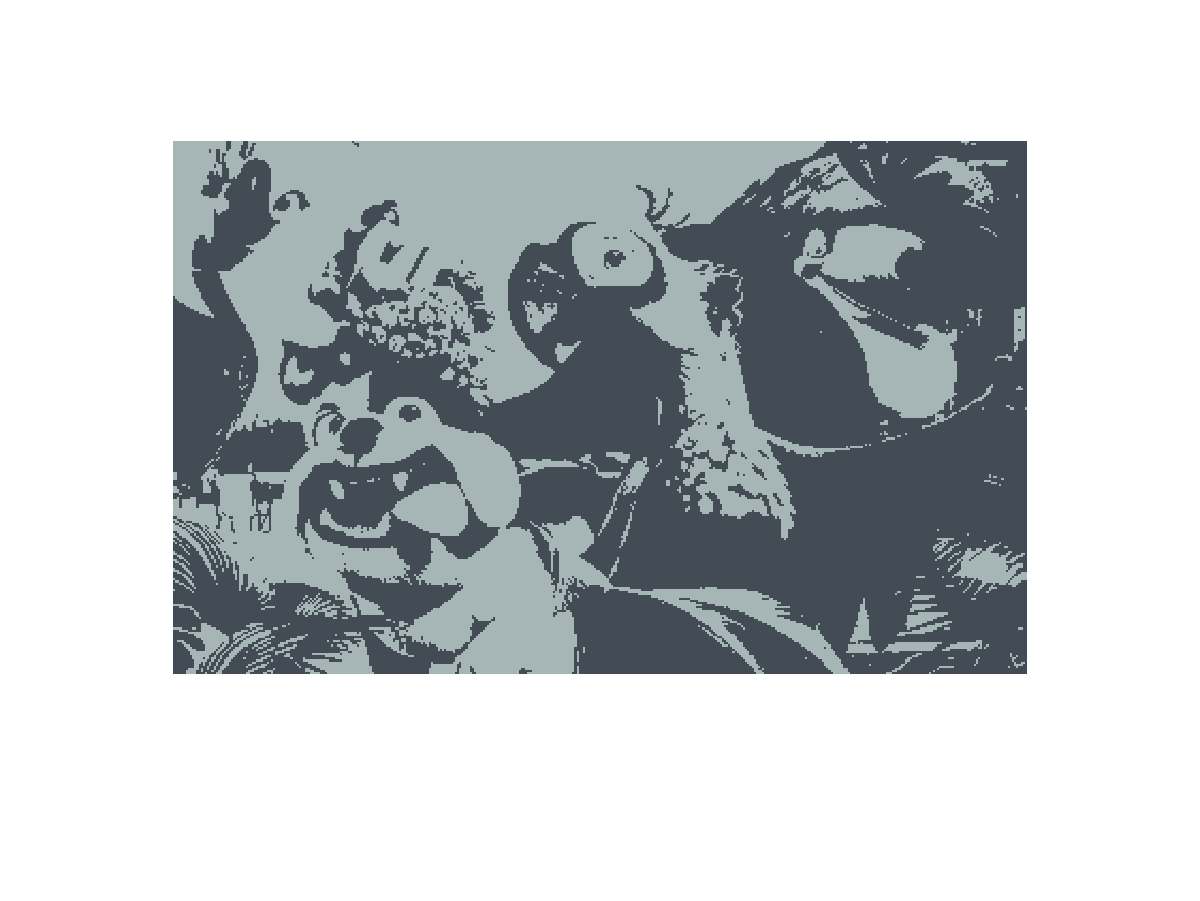
\includegraphics[scale=0.4]{./pics/task1and2/rio_k=2_random/K=2_iteration_10_random_2_rio.png} \\\hline
  \end{longtable}	
\end{center}

\myparagraph{final segmented image}

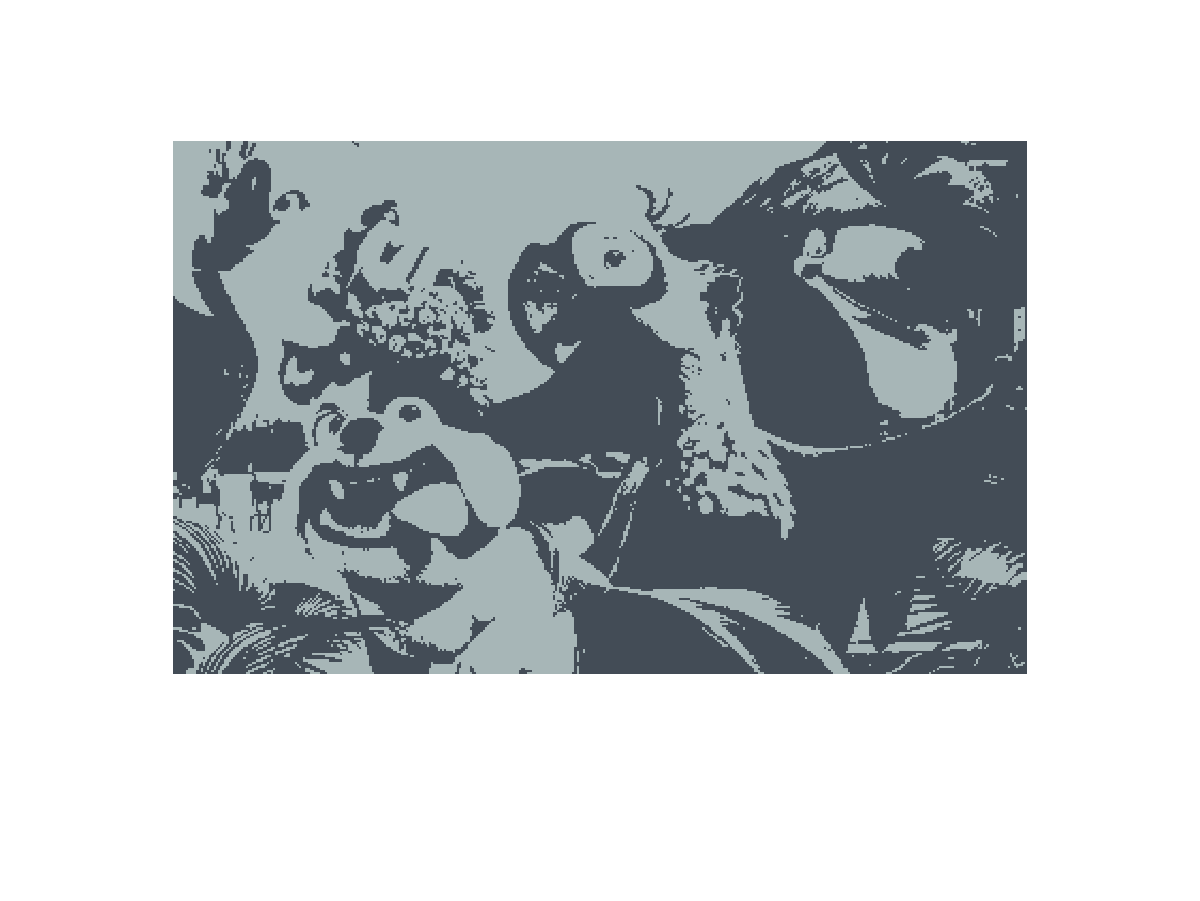
\includegraphics[scale=0.4]{./pics/task1and2/rio_k=2_random/K=2_iteration_17_random_2_rio.png}\\

\begin{center}
  \begin{longtable}{ c | c }
	\multicolumn{1}{c}{iteration vs. cost} & 
	\multicolumn{1}{c}{iteration vs. cluster assignment changes}  \\
    \hline
    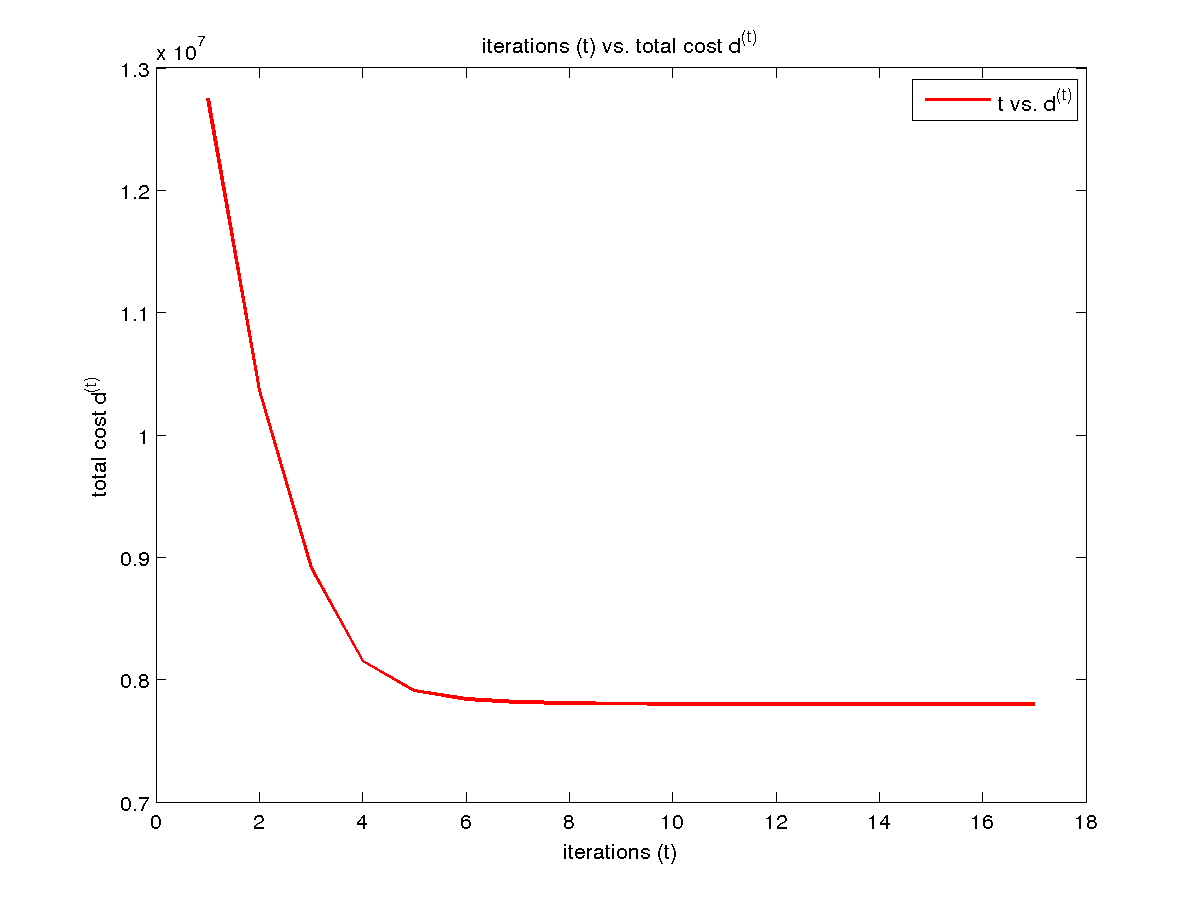
\includegraphics[scale=0.4]{./pics/task1and2/rio_k=2_random/t_vs_d_random_2_rio.png}  & 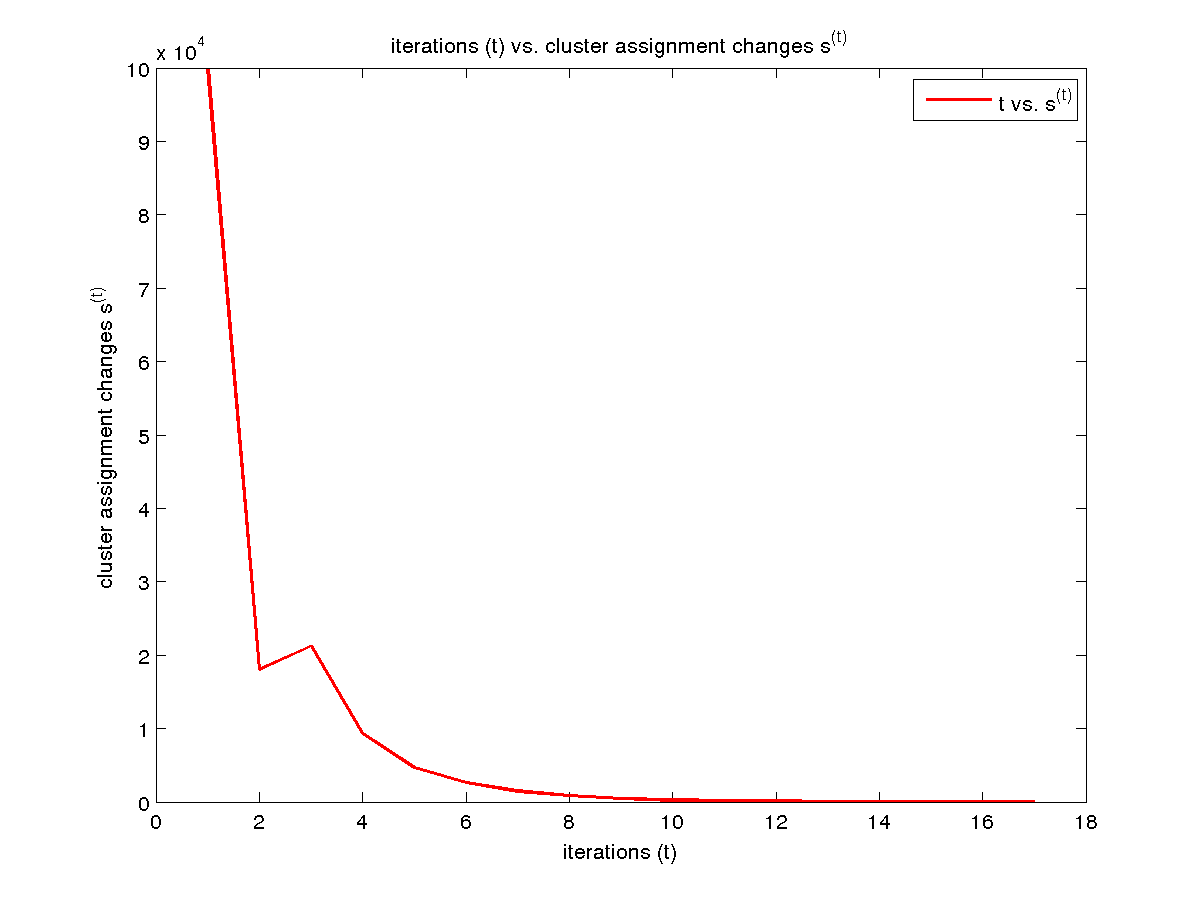
\includegraphics[scale=0.4]{./pics/task1and2/rio_k=2_random/t_vs_s_random_2_rio.png} \\
    \hline
  \end{longtable}
\end{center}

\subsubsection{number of clusters = 4}

\begin{center}
  \begin{longtable}{ c | c }
	\multicolumn{1}{c}{} & 
	\multicolumn{1}{c}{}  \\
	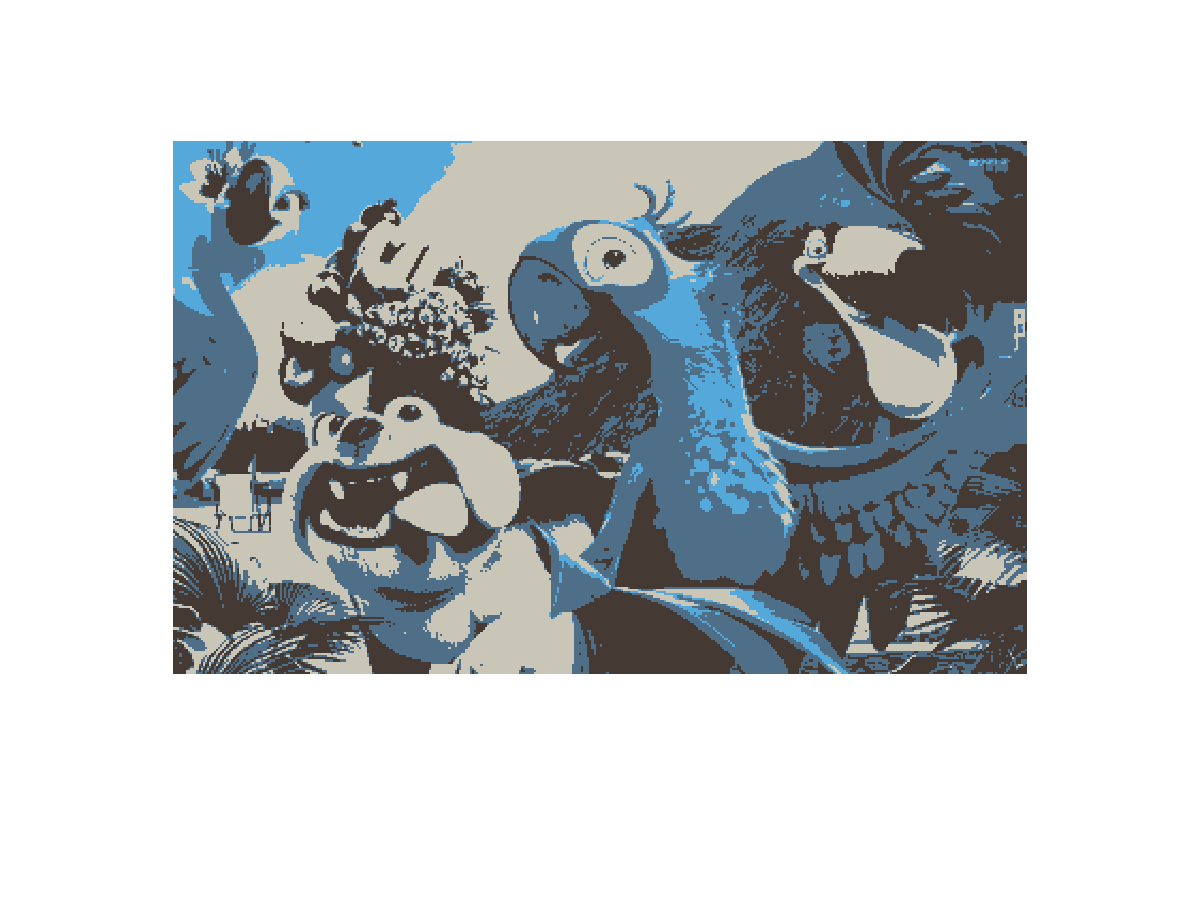
\includegraphics[scale=0.4]{./pics/task1and2/rio_k=4_random/K=4_iteration_1_random_4_rio.png} & 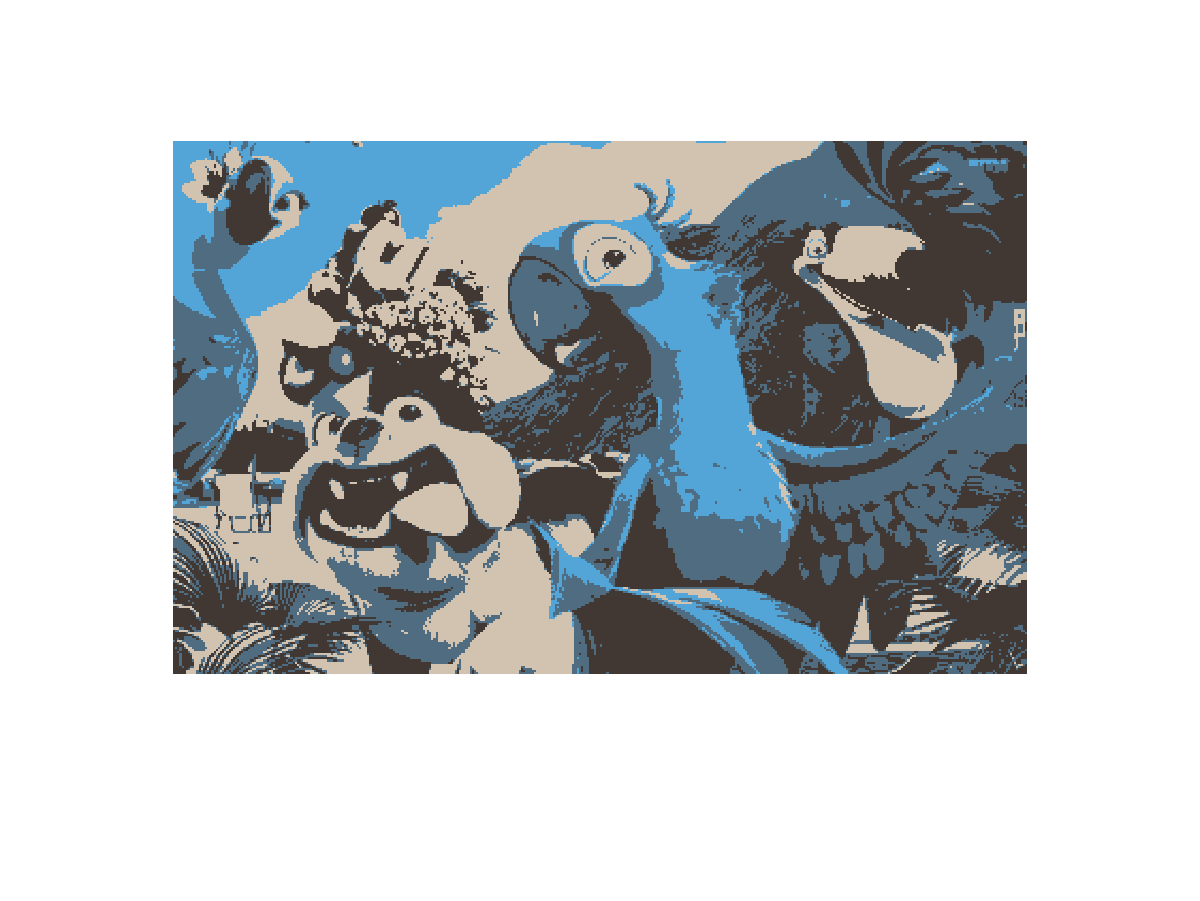
\includegraphics[scale=0.4]{./pics/task1and2/rio_k=4_random/K=4_iteration_2_random_4_rio.png} \\\hline
	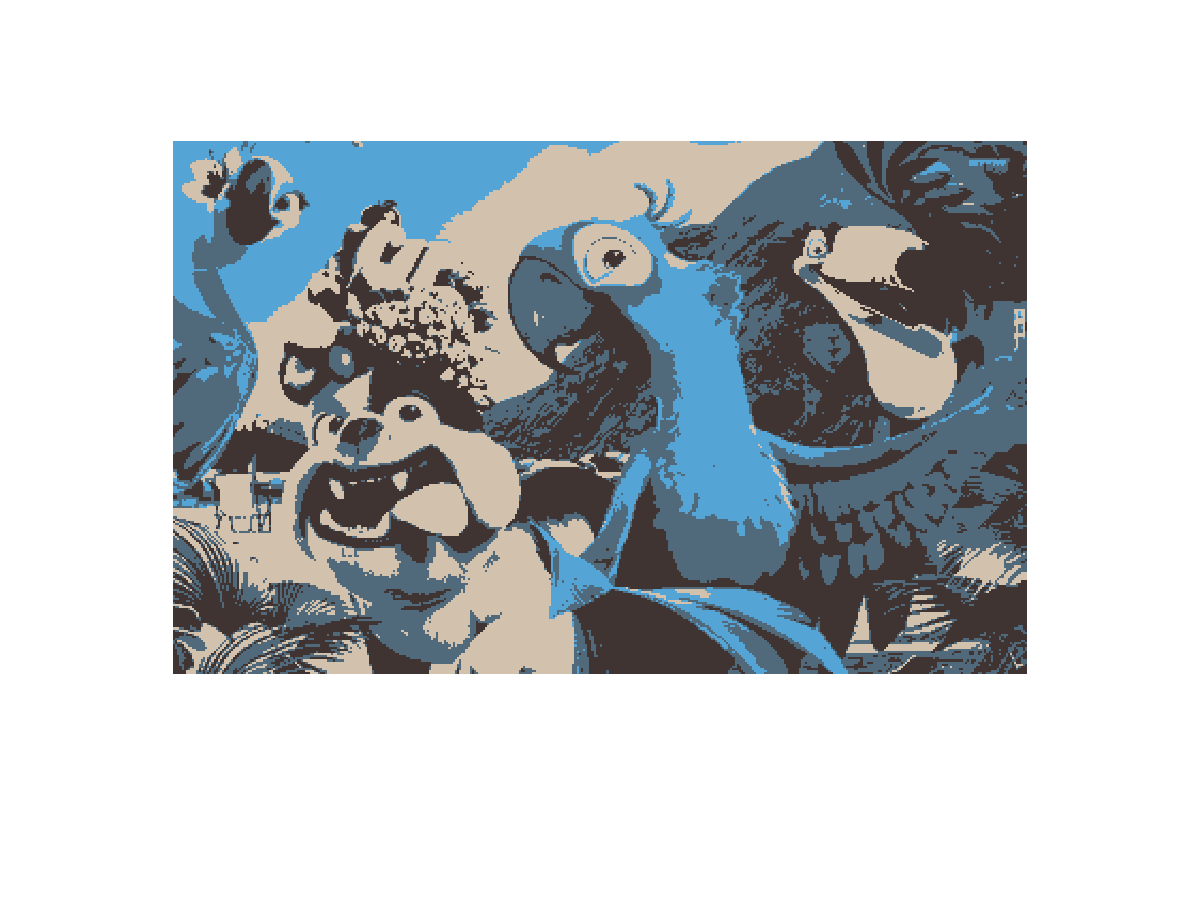
\includegraphics[scale=0.4]{./pics/task1and2/rio_k=4_random/K=4_iteration_3_random_4_rio.png} & 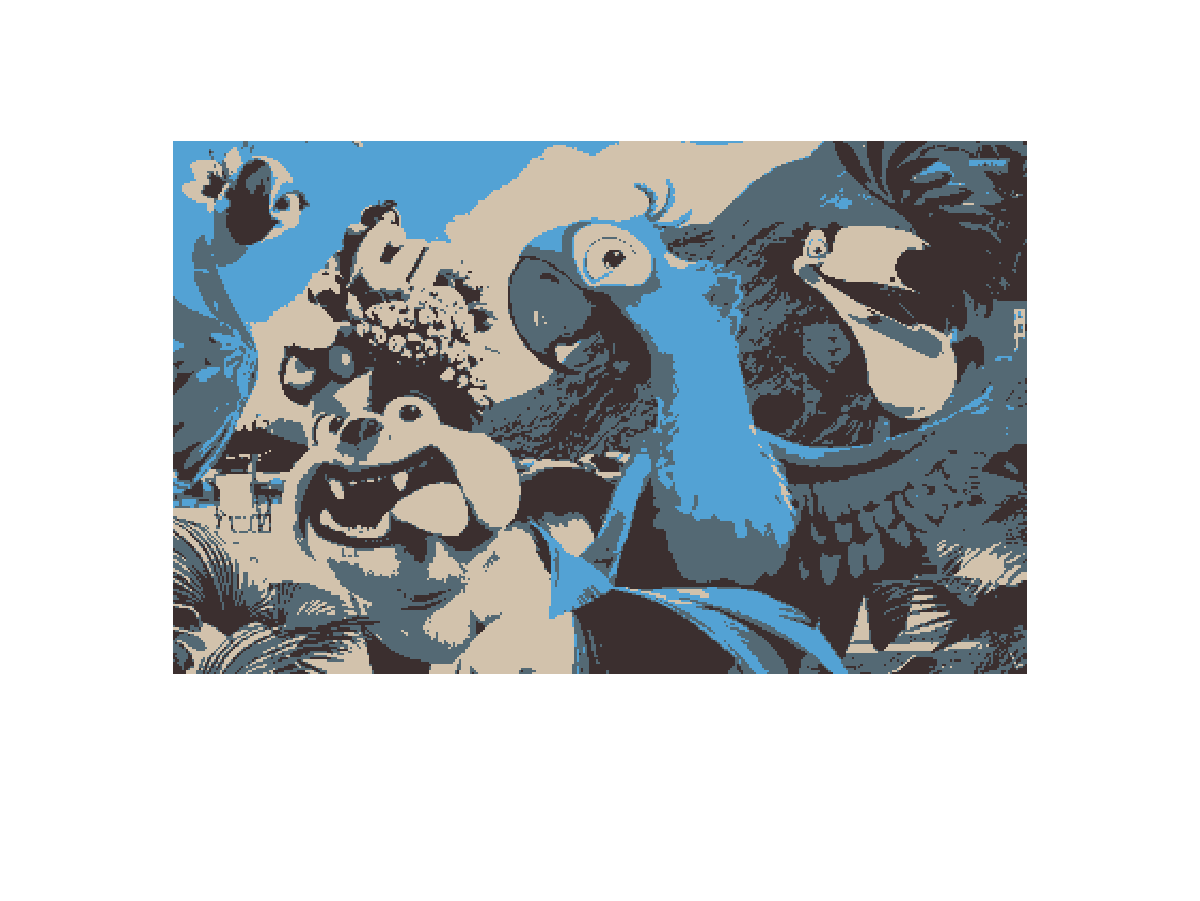
\includegraphics[scale=0.4]{./pics/task1and2/rio_k=4_random/K=4_iteration_4_random_4_rio.png} \\\hline
	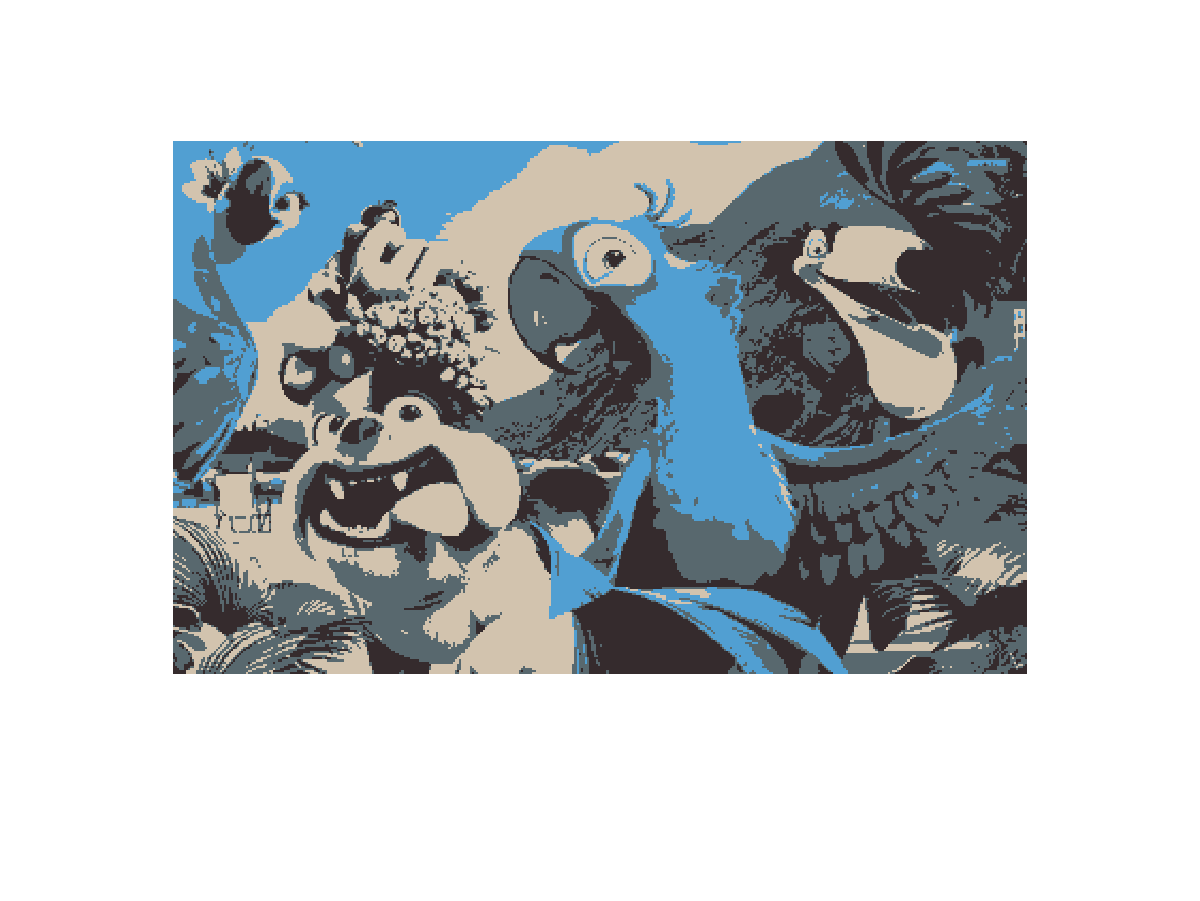
\includegraphics[scale=0.4]{./pics/task1and2/rio_k=4_random/K=4_iteration_5_random_4_rio.png} & 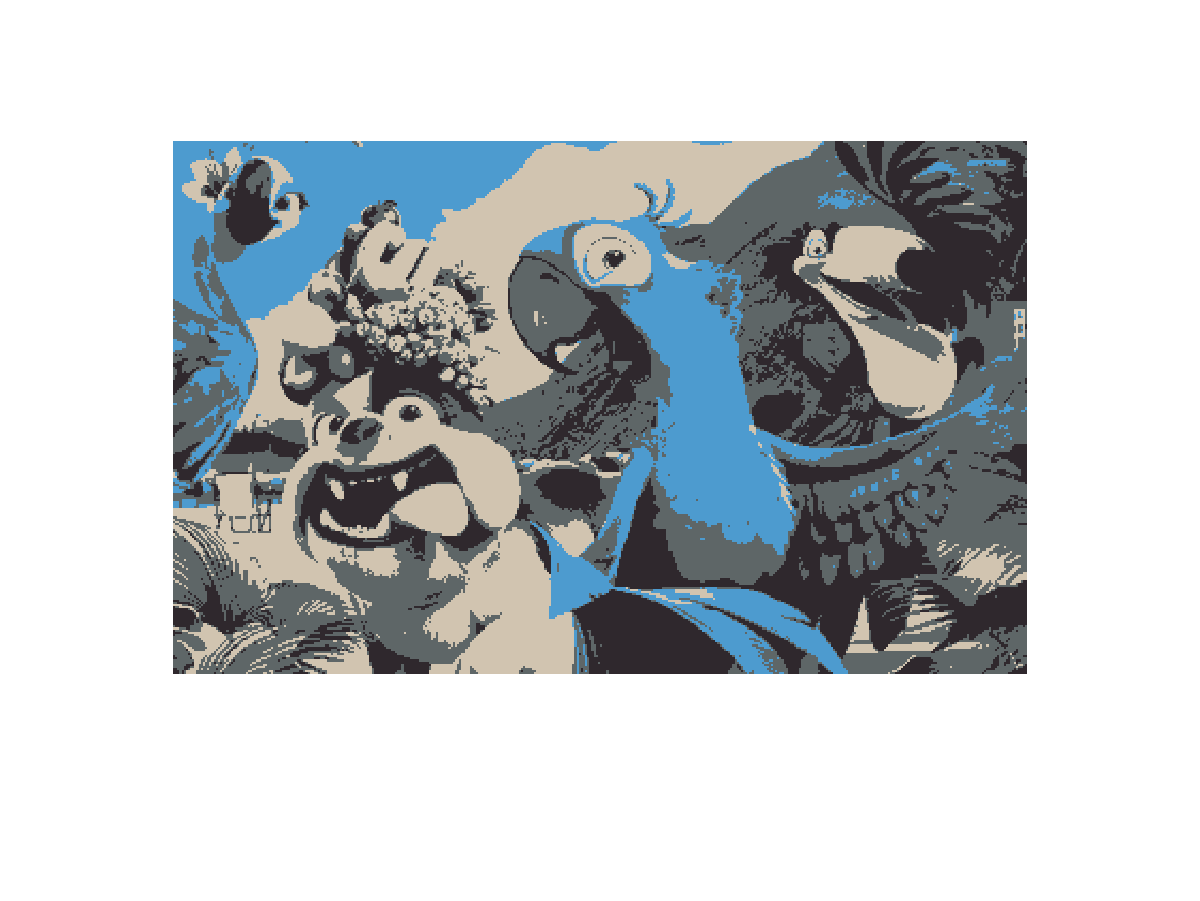
\includegraphics[scale=0.4]{./pics/task1and2/rio_k=4_random/K=4_iteration_6_random_4_rio.png} \\\hline
	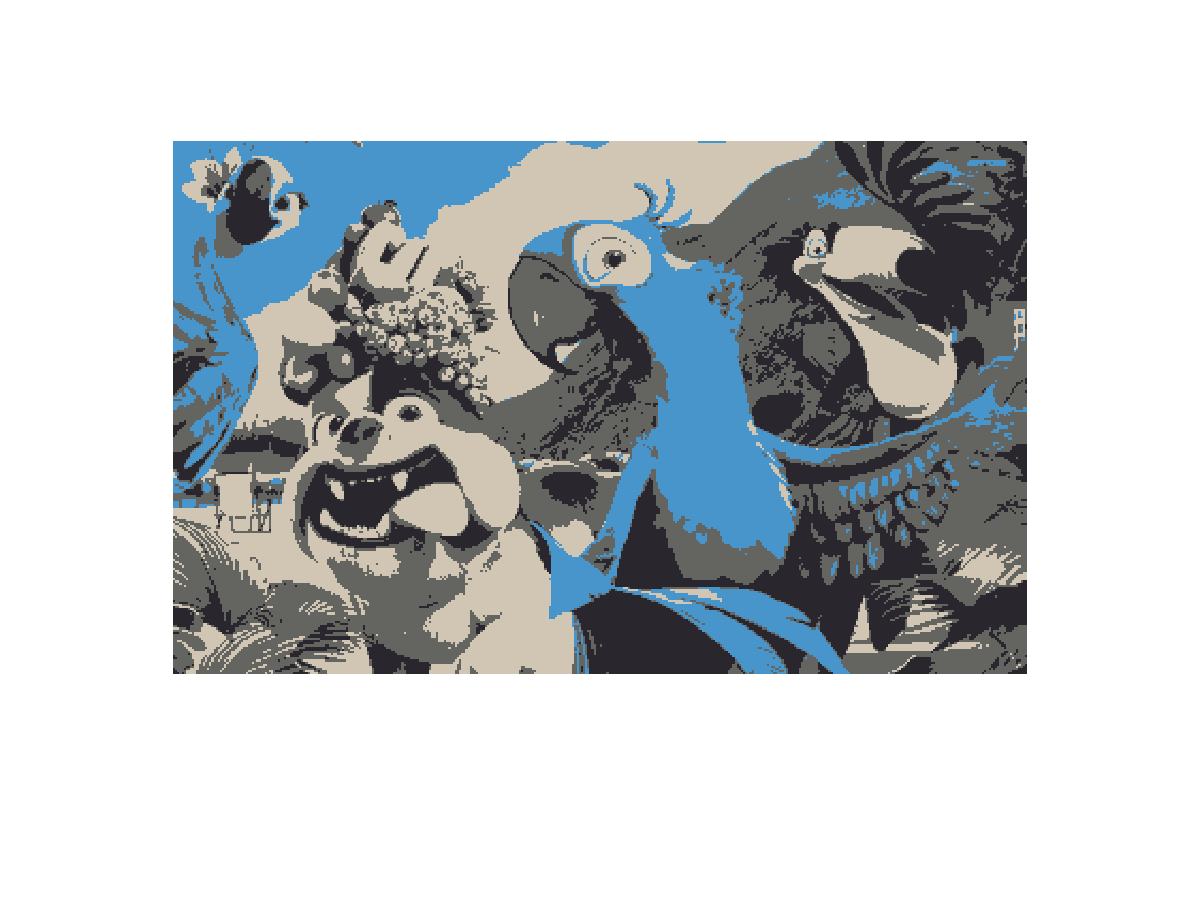
\includegraphics[scale=0.4]{./pics/task1and2/rio_k=4_random/K=4_iteration_7_random_4_rio.png} & 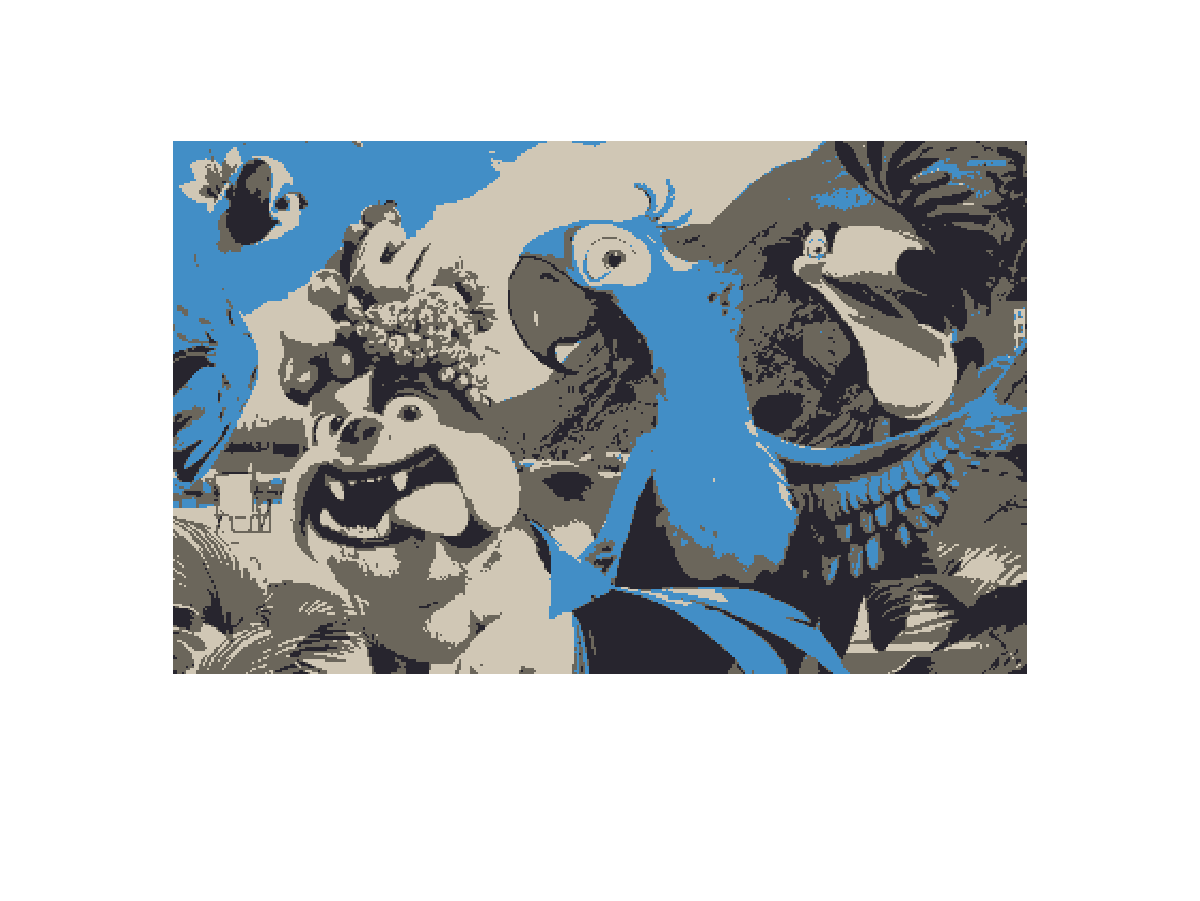
\includegraphics[scale=0.4]{./pics/task1and2/rio_k=4_random/K=4_iteration_8_random_4_rio.png} \\\hline
	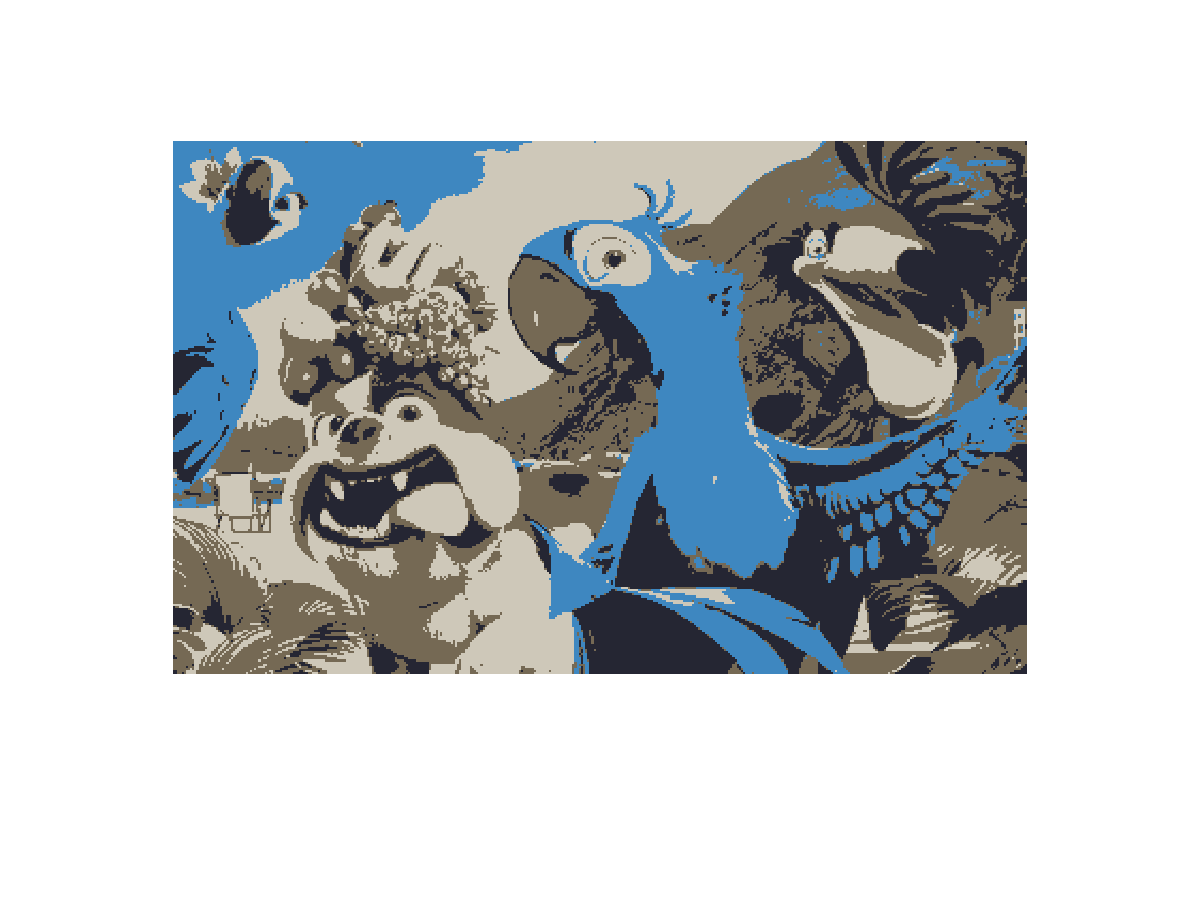
\includegraphics[scale=0.4]{./pics/task1and2/rio_k=4_random/K=4_iteration_9_random_4_rio.png} & 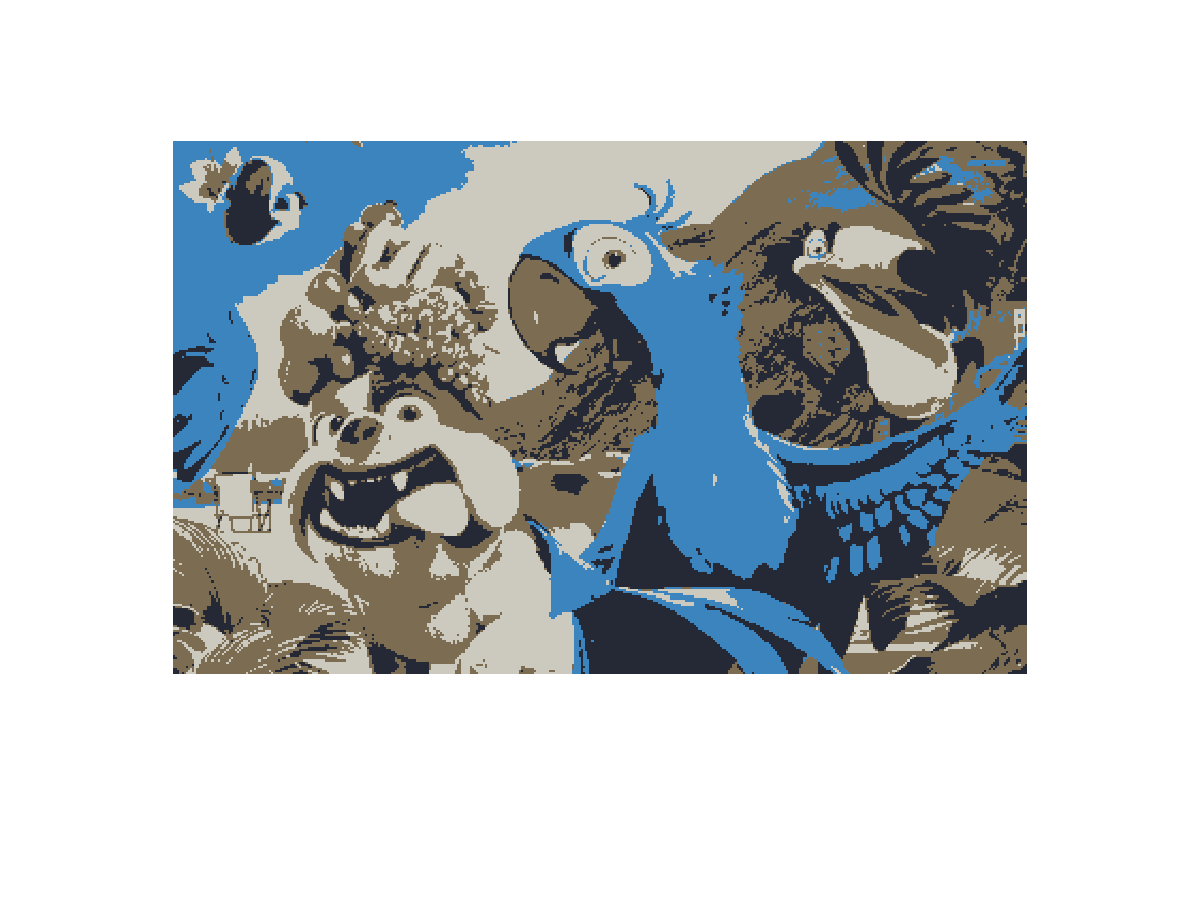
\includegraphics[scale=0.4]{./pics/task1and2/rio_k=4_random/K=4_iteration_10_random_4_rio.png} \\\hline
  \end{longtable}	
\end{center}

\myparagraph{final segmented image}

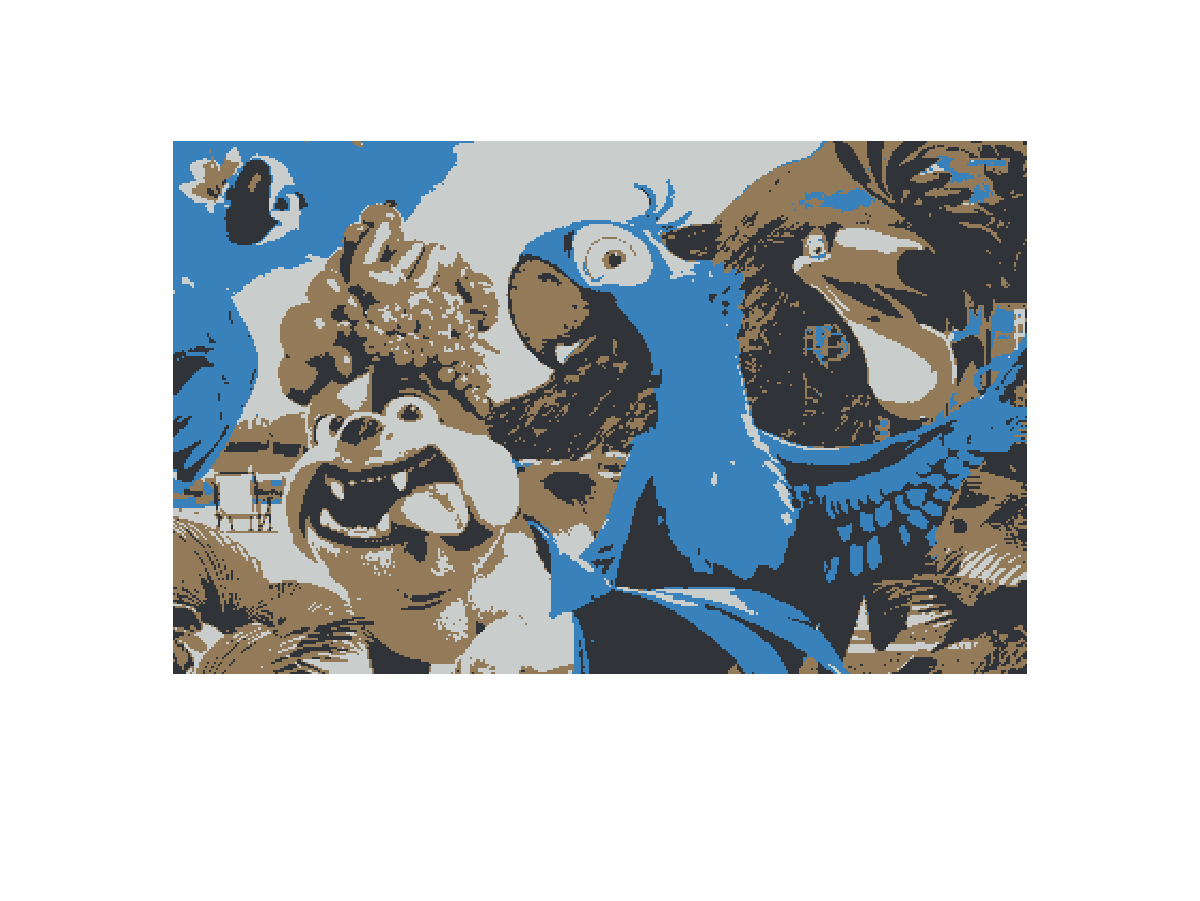
\includegraphics[scale=0.4]{./pics/task1and2/rio_k=4_random/K=4_iteration_51_random_4_rio.png}\\
\begin{center}
  \begin{longtable}{ c | c }
	\multicolumn{1}{c}{iteration vs. cost} & 
	\multicolumn{1}{c}{iteration vs. cluster assignment changes}  \\
    \hline
    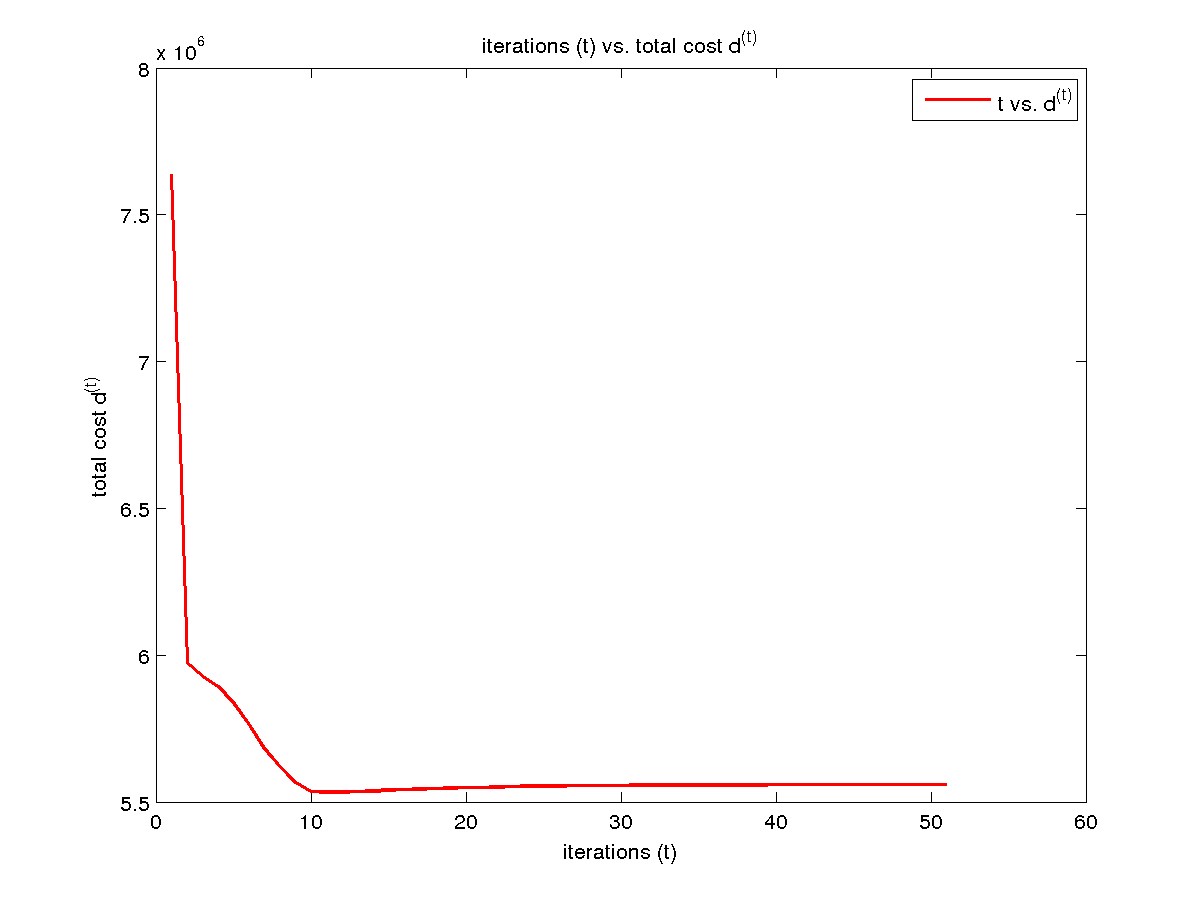
\includegraphics[scale=0.4]{./pics/task1and2/rio_k=4_random/t_vs_d_random_4_rio.png}  & 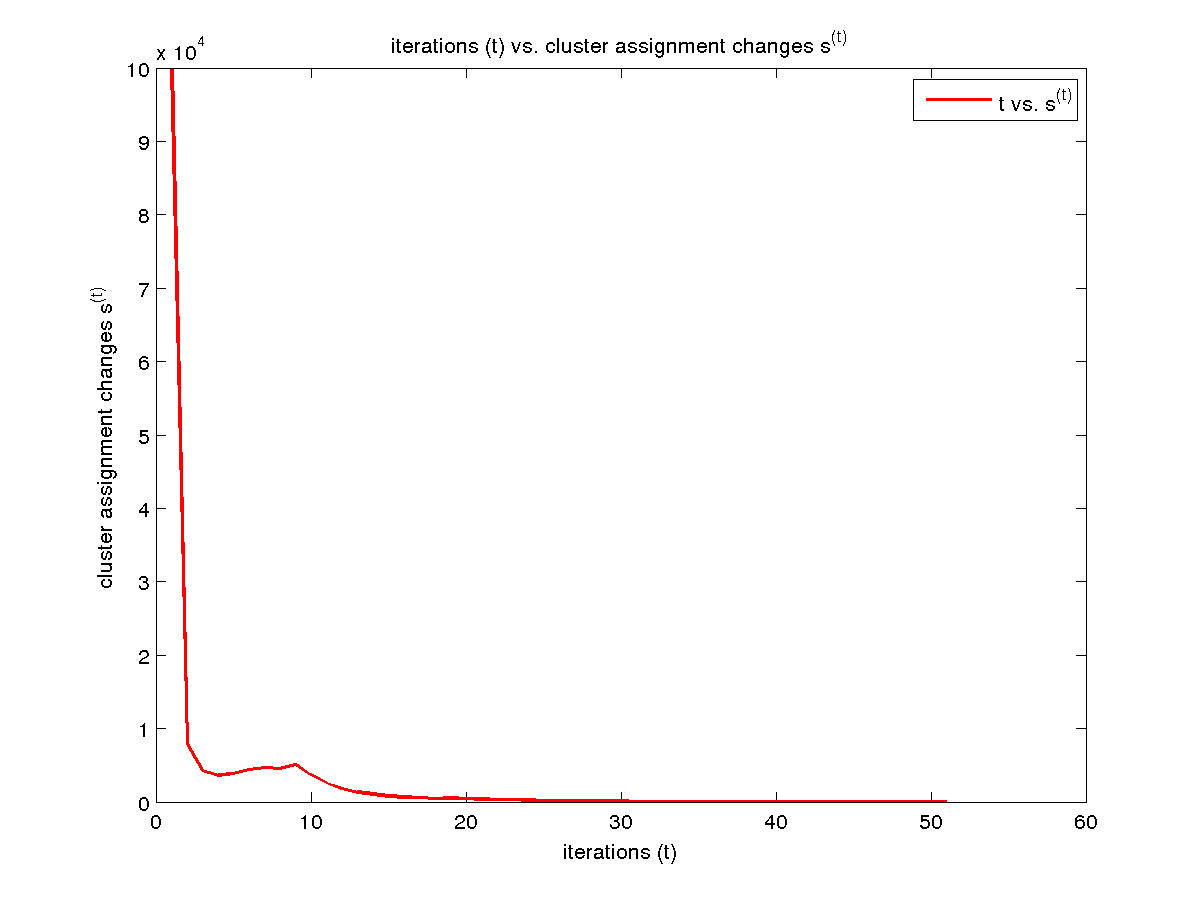
\includegraphics[scale=0.4]{./pics/task1and2/rio_k=4_random/t_vs_s_random_4_rio.png} \\
    \hline
  \end{longtable}
\end{center}

\subsubsection{number of clusters = 8}
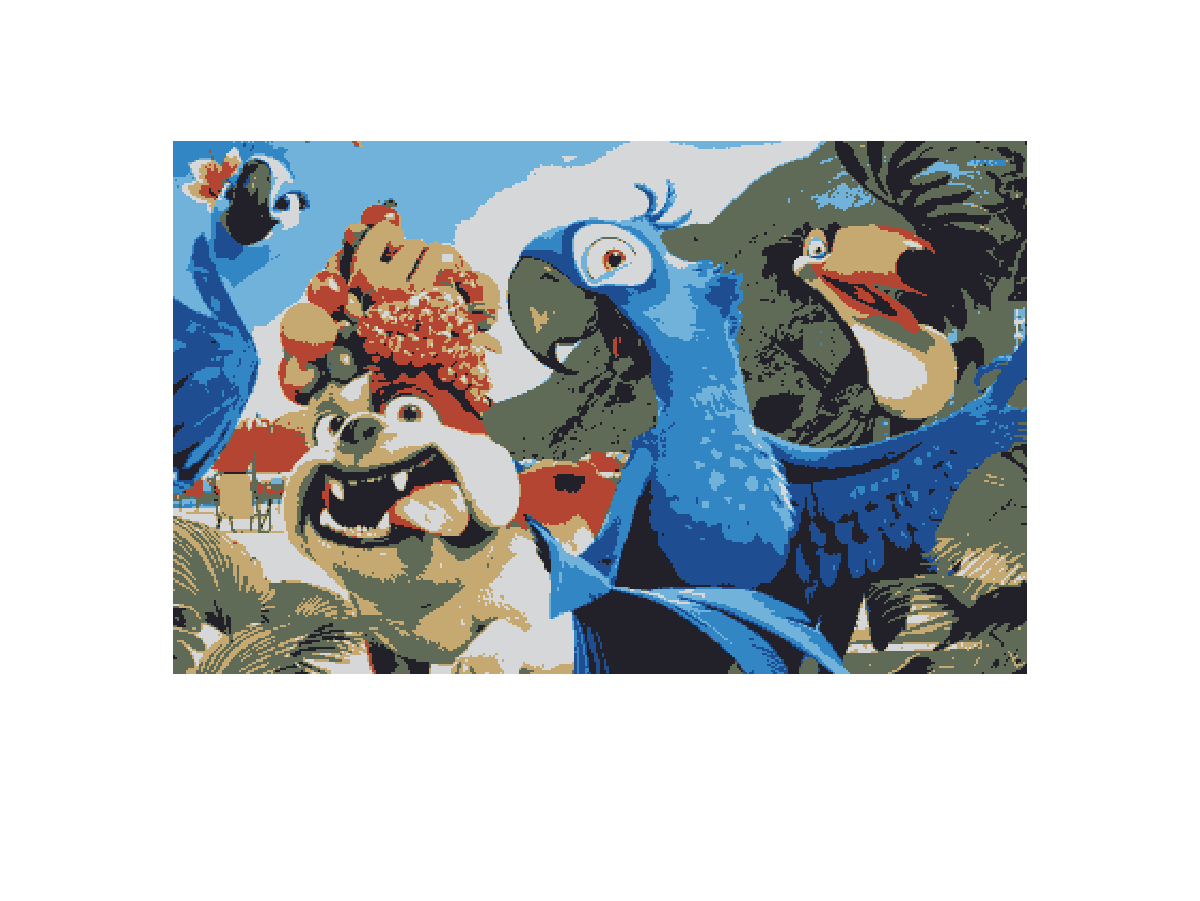
\includegraphics[scale=0.4]{./pics/task1and2/rio_k=8_random/K=8_iteration_79_random_8_rio.png}\\
\begin{center}
  \begin{longtable}{ c | c }
	\multicolumn{1}{c}{iteration vs. cost} & 
	\multicolumn{1}{c}{iteration vs. cluster assignment changes}  \\
    \hline
    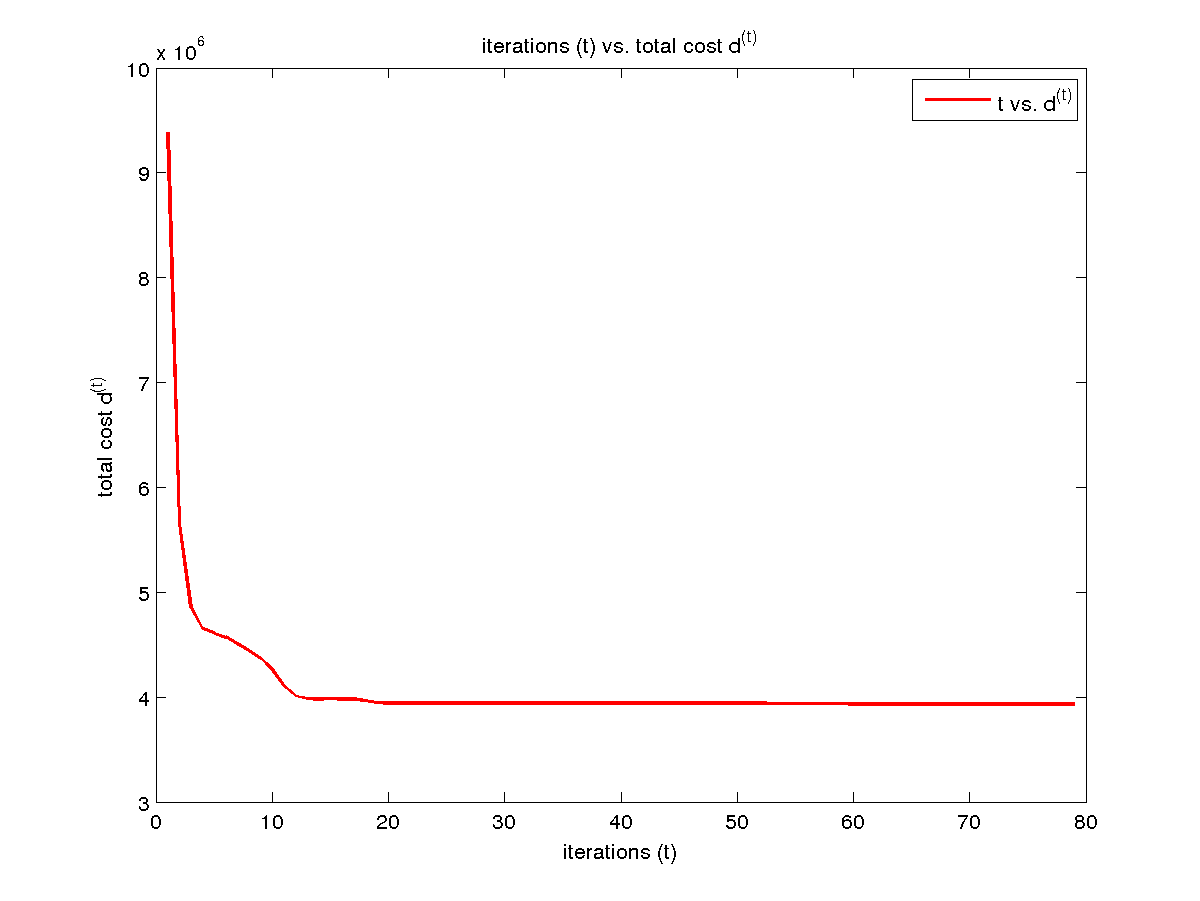
\includegraphics[scale=0.4]{./pics/task1and2/rio_k=8_random/t_vs_d_random_8_rio.png}  & 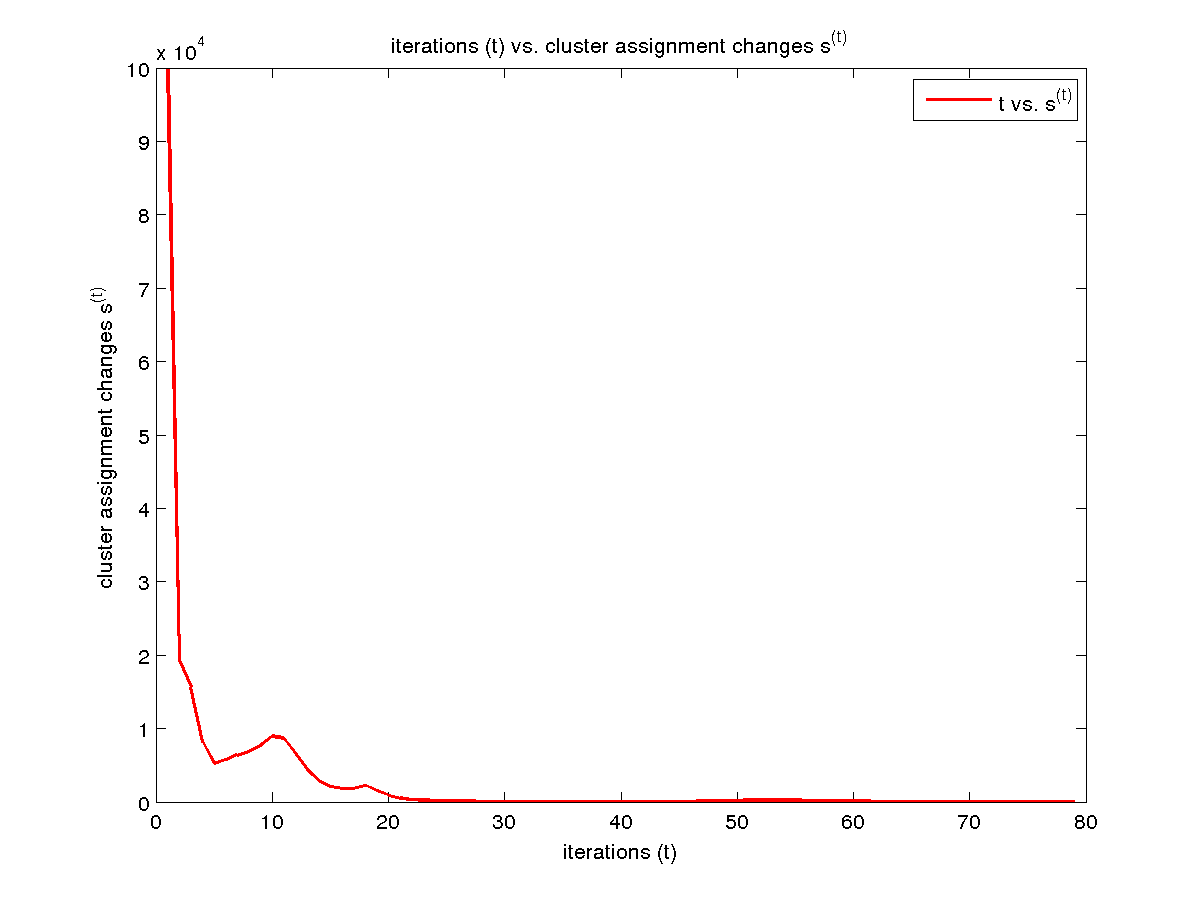
\includegraphics[scale=0.4]{./pics/task1and2/rio_k=8_random/t_vs_s_random_8_rio.png} \\
    \hline
  \end{longtable}
\end{center}

\subsubsection{K-means algorithm - general property}

K-means clustering algorithm guarantees only a local minimum (the local minimum is dependent on the random initialization of means).\\

\newpage
\section{Image segmentation using Gaussian mixture model (EM algorithm)}

\subsection{spectrum.png with K=7}
\subsubsection{Random initializations}
\begin{center}
  \begin{longtable}{ c | c }
	\multicolumn{1}{c}{Random initialization-1} & 
	\multicolumn{1}{c}{Random initialization-2}  \\
    \hline
    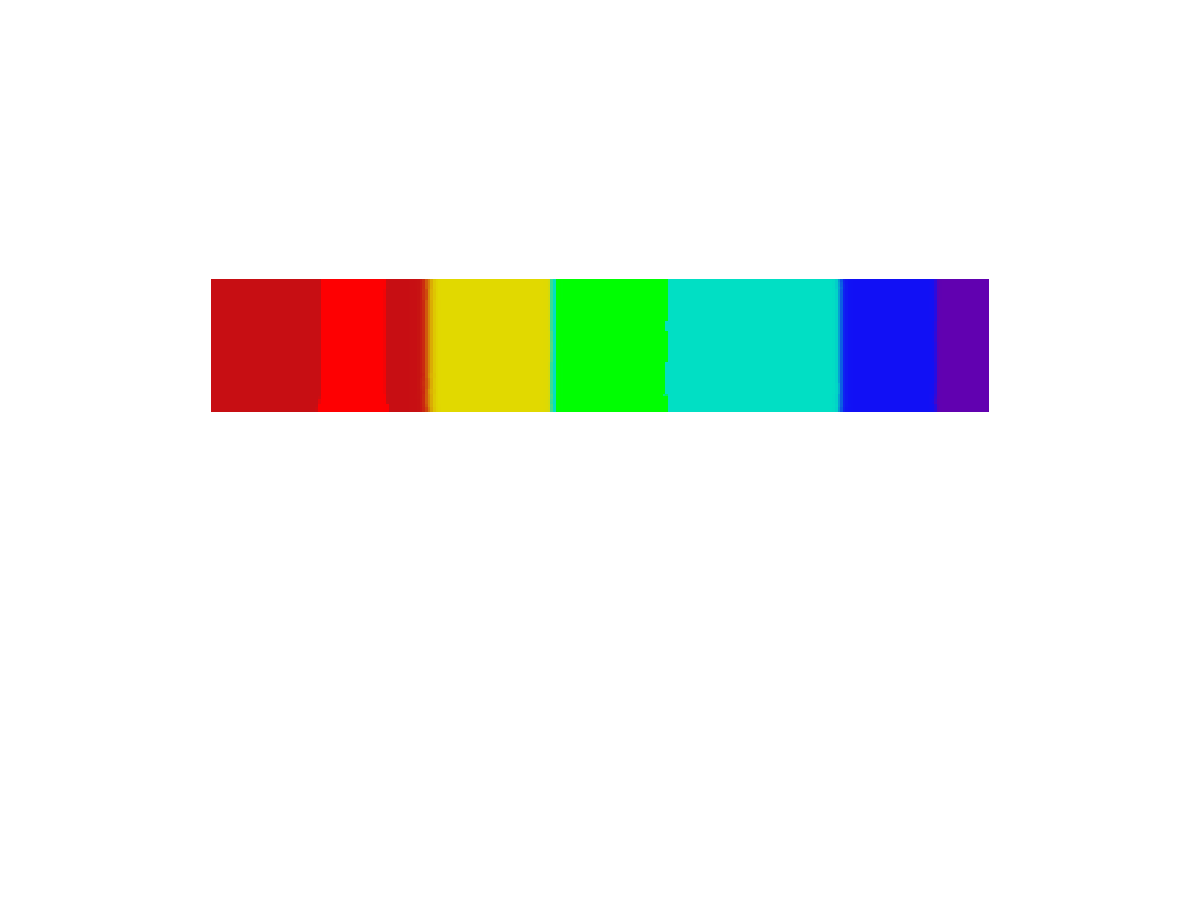
\includegraphics[scale=0.4]{./pics/task1and2/EM_K=7_spectrum_random1.png}  & 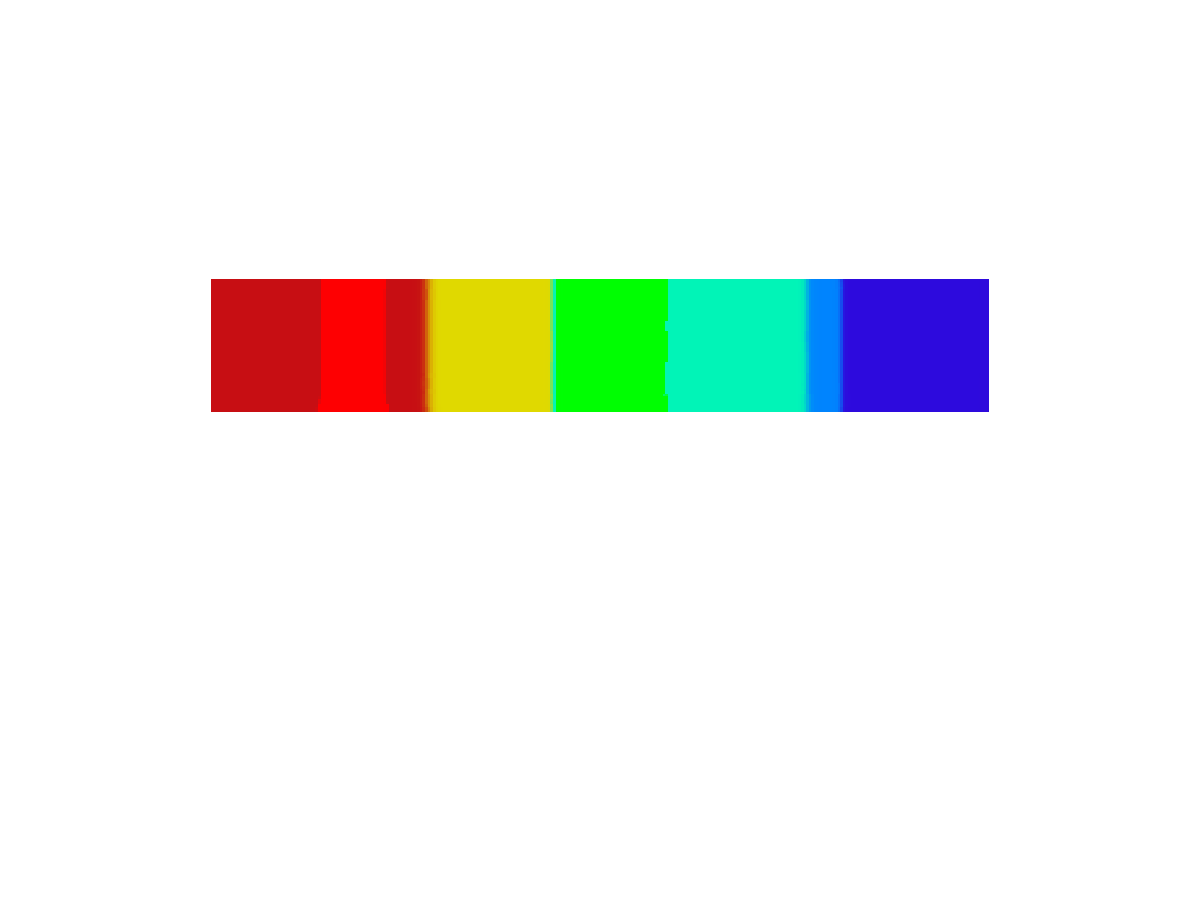
\includegraphics[scale=0.4]{./pics/task1and2/EM_K=7_spectrum_random2.png} \\
    \hline
  \end{longtable}
\end{center}

\subsection{rio.png with K=8}
\subsubsection{Random initializations}
\begin{center}
  \begin{longtable}{ c | c }
	\multicolumn{1}{c}{Random initialization-1} & 
	\multicolumn{1}{c}{Random initialization-2}  \\
    \hline
    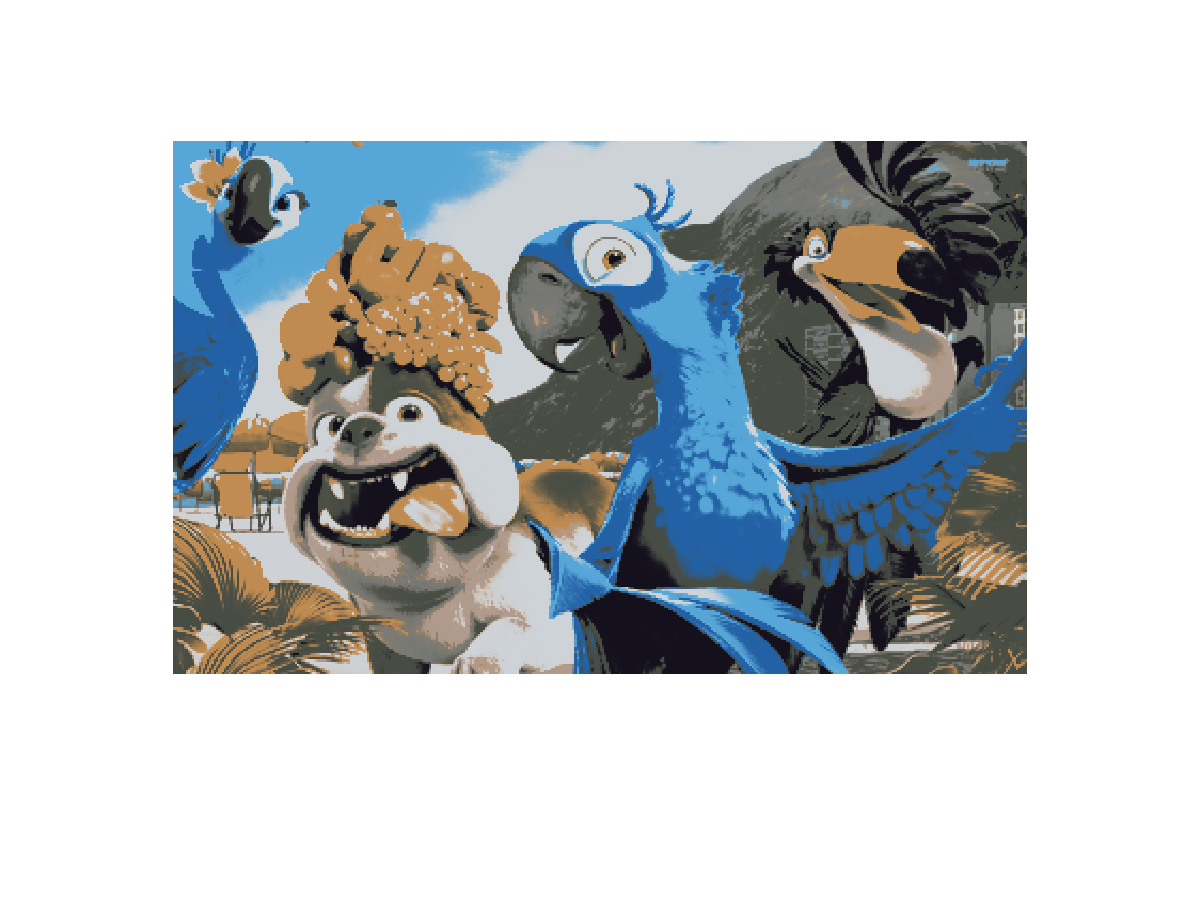
\includegraphics[scale=0.4]{./pics/task1and2/EM_K=8_rio_random1.png}  & 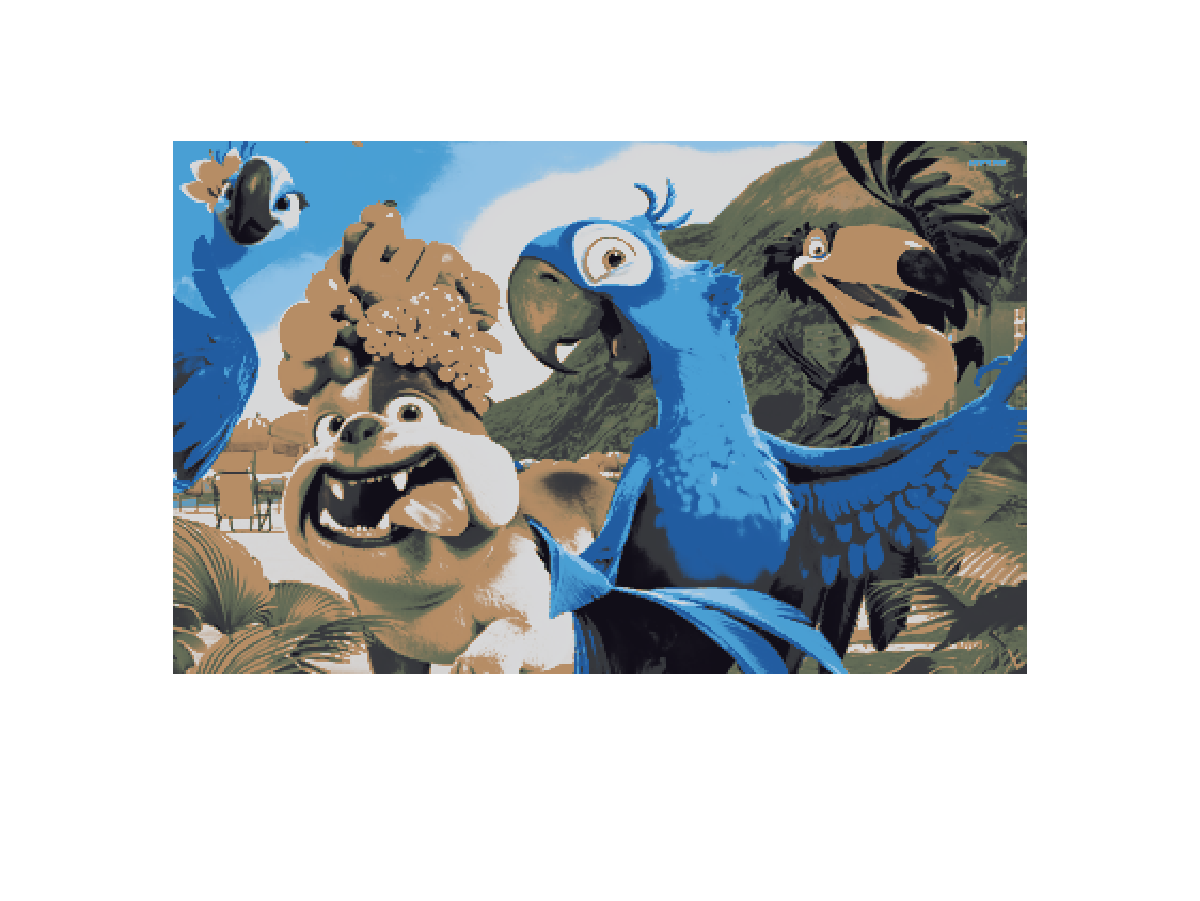
\includegraphics[scale=0.4]{./pics/task1and2/EM_K=8_rio_random2.png} \\
    \hline
  \end{longtable}
\end{center}

\subsection{Difference between K-means clustering \& EM algorithms (e.g., GMM)}

\begin{itemize}
	\item K-means clustering algorithm follows Hard clustering policy in which a particular datapoint is assigned to a cluster completely, where as 
	in EM algorthms such as Gaussian Mixture Model, any data point is assigned to multiple clusters (soft assignment) with a probabilistic weightage.
	\item K-means clustering algorithm tends to use less number of parameters than EM algorithms. Considering K-means and GMM, 
	K-means algorithm uses K number of means, where as GMM uses K number of means + K number of weight parameters, K number of $dxd$ covariance matrices.
\end{itemize}

\newpage
\section{Linear regression}
\subsection{Maximum likelihood method}
Let $X=[x_1 x_2 \ldots x_I]$ be the data examples given. ($x_i = [1 x']$)\\\\
we can define that, P($w_i|x_i$) = $N_w(\phi^Tx_i, \sigma^2)$. \\\\
ML estimate of $\phi$ is given by, $\phi_{ML}$ = $(XX^T)^{-1}Xw$

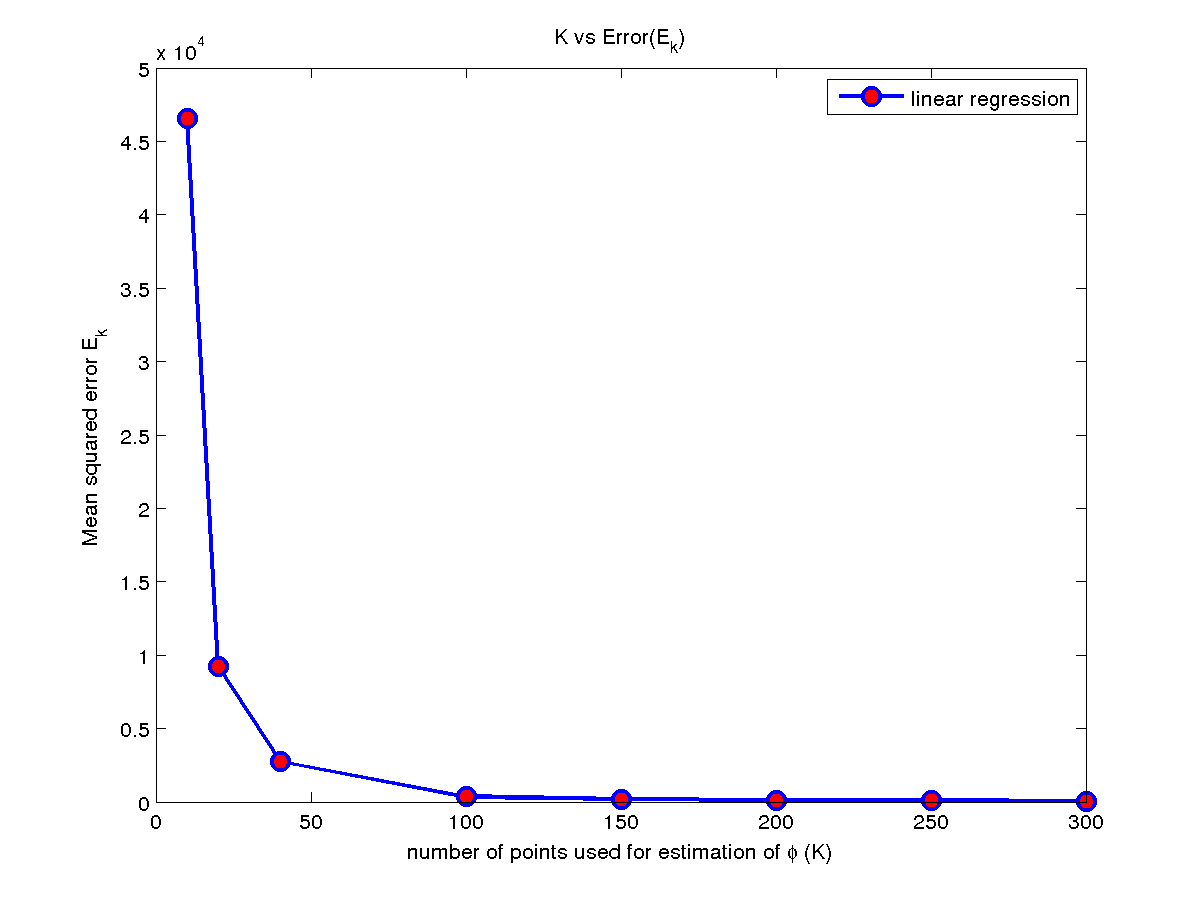
\includegraphics[scale=0.6]{./pics/task3/linear_regression_error_vs_k.png}

\subsection{Bayesian regression method}

Posterior distribution P($\phi | w, X$) =  ${P(w|X,\phi) P(\phi)}\over{P(w|X)}$\\\\
here, the likelihood is given by $P(w|X, \theta) = N_w(X^T\phi, \sigma^2)$.\\\\
hence, $P(\phi|X,w) = N_{\phi}({{A^{-1}Xw} \over {\sigma^2}}, A^{-1})$, where A = ${{XX^T}\over{\sigma^2}} + {I\over\sigma_{p}^2}$ \\\\
Predictive distribution is given by, $P(w^*|x^*, X, w) = N_{w^*}({{x^{*T}A^{-1}Xw}\over{\sigma^2}}, {x^{*T}A^{-1}x^*})$

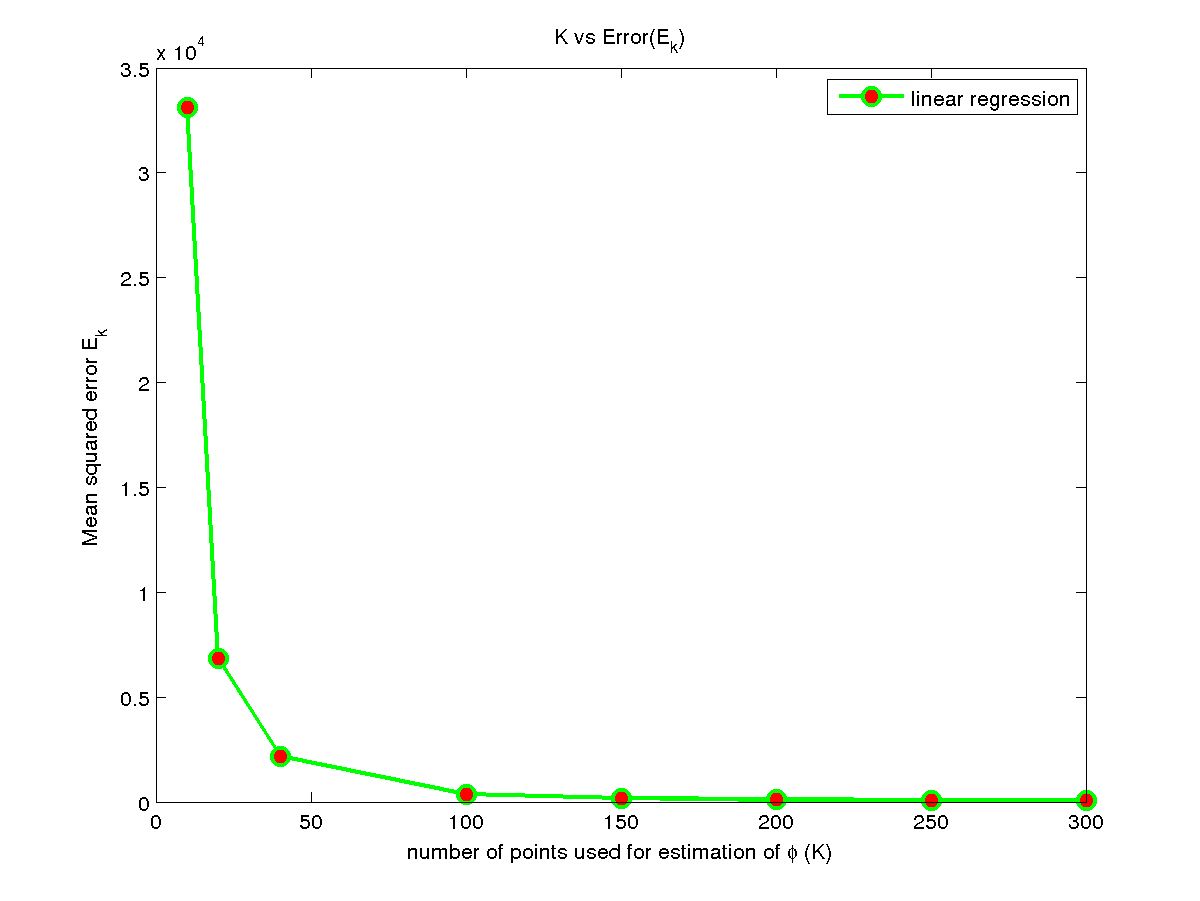
\includegraphics[scale=0.6]{./pics/task3/bayes_regression_error_vs_k.png}

\subsection{Comparision}
As seen in the image below, the ML estimate is giving high MSE when less number of points are used in Regression. 
When the number of points are increased, the error of ML estimate converges with Bayesian estimate.

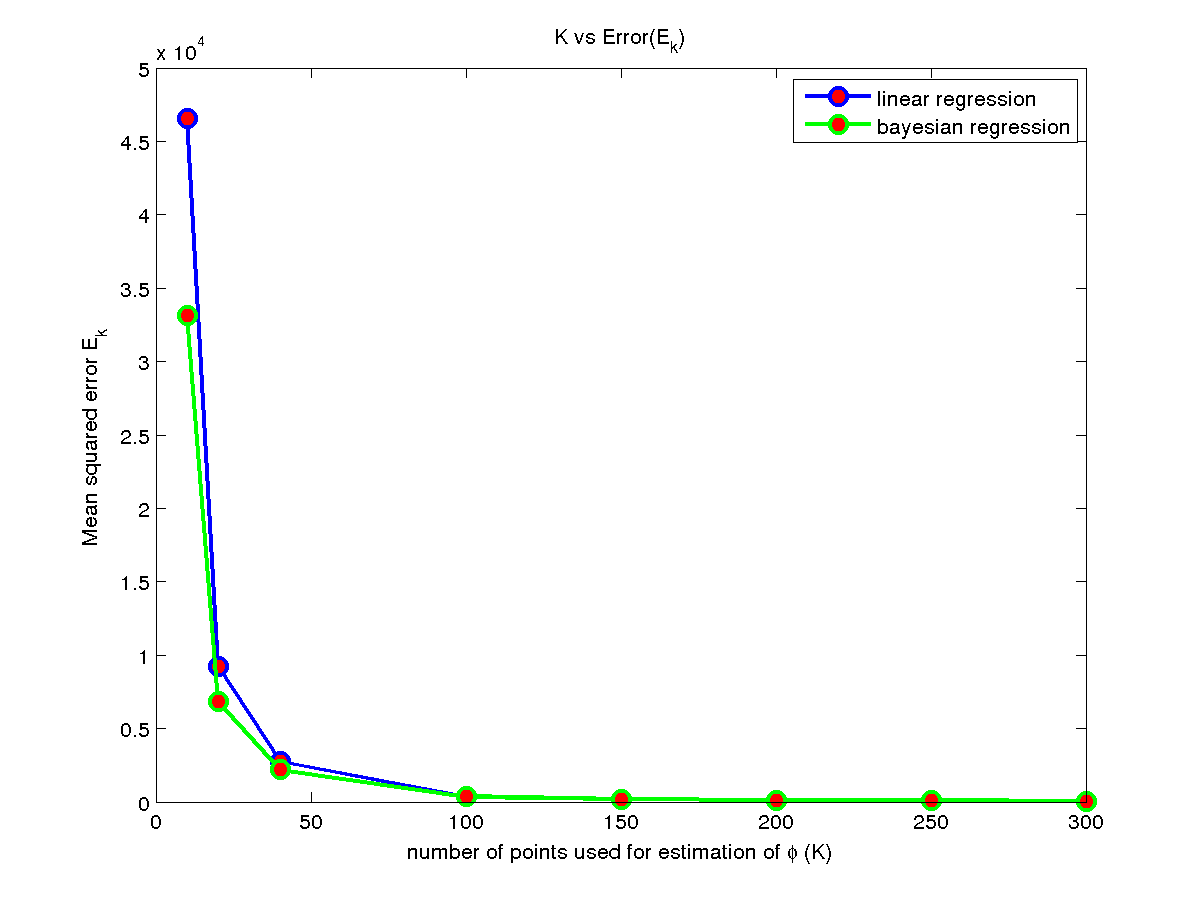
\includegraphics[scale=0.6]{./pics/task3/linear_bayes_regression_error_vs_k.png}

\newpage
\section{Non-linear regression}
\subsection{Data}
By looking at the data, it shall be inferred that the Linear regression methods (involving linear terms of Data $x$) will not be sufficient to model the data, as Data seems to involve non-linear characteristics.\\\\
To model the data well, we need to go for Non-linear regression where we involve non-linear terms ($x^2, x^3, \ldots, gaussian, arctan$). 
\begin{center}
  \begin{longtable}{ c | c }
	\multicolumn{1}{c}{Ground truth} & 
	\multicolumn{1}{c}{Noise-added data}  \\
    \hline
    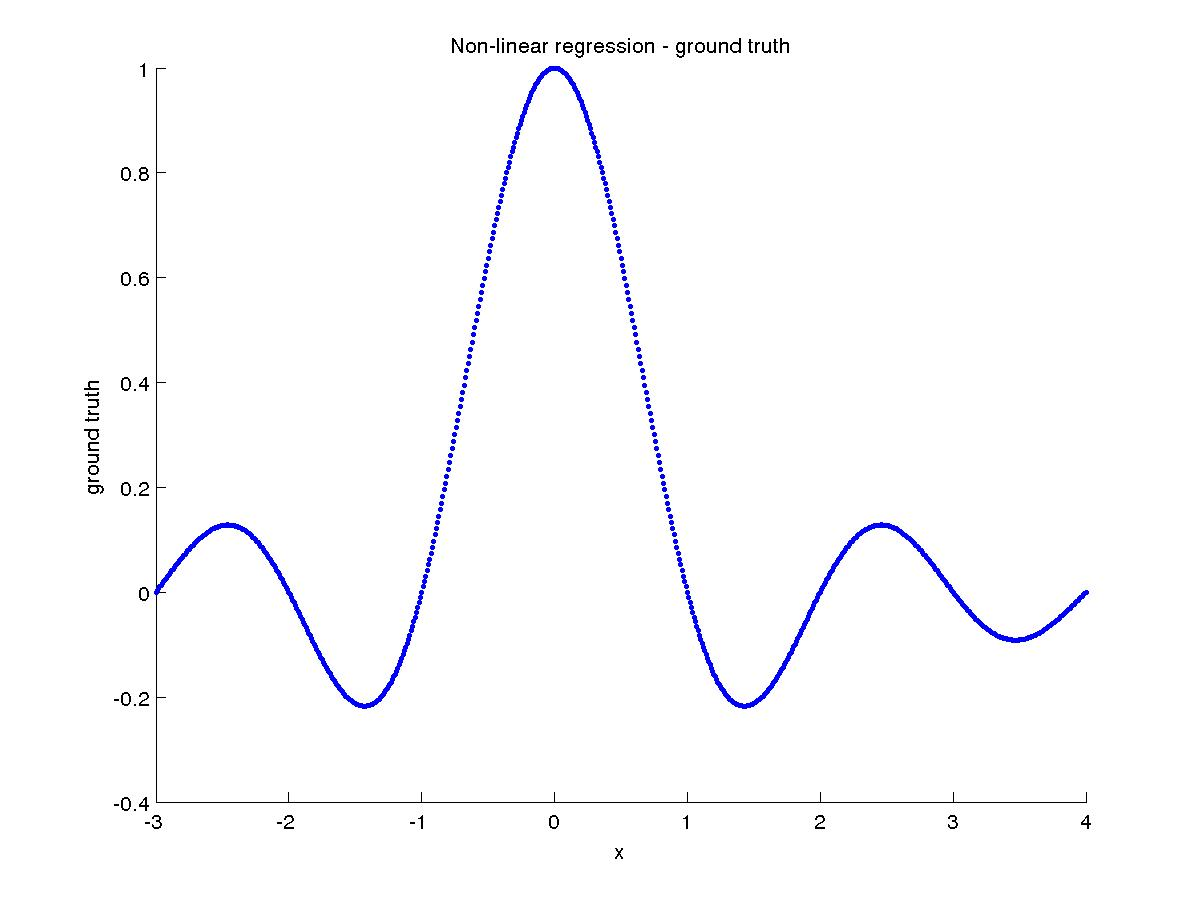
\includegraphics[scale=0.2]{./pics/task4/ground_truth.jpg}  & 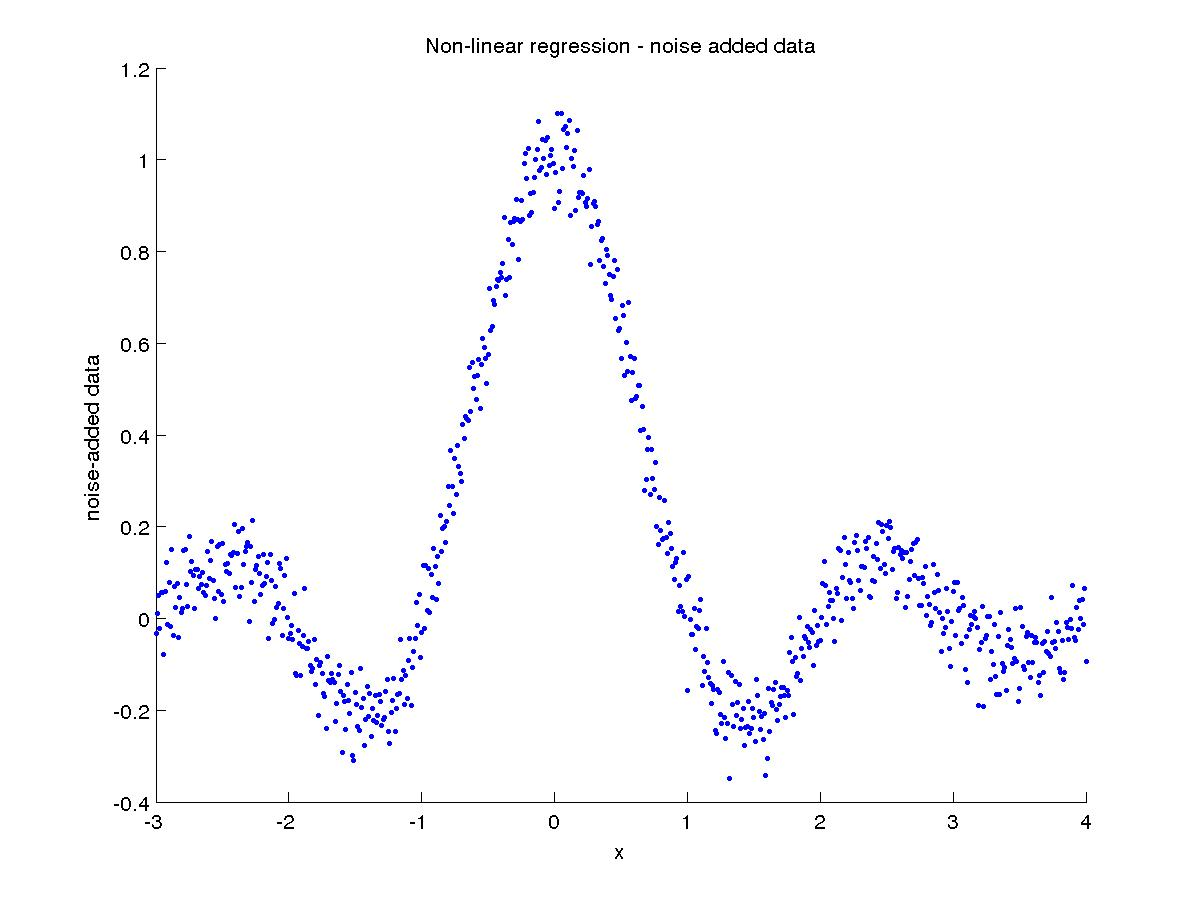
\includegraphics[scale=0.2]{./pics/task4/noise_added_data.jpg} \\
    \hline
  \end{longtable}
\end{center}

\subsection{RBF with 6 kernel functions}
with 6 RBF kernel functions, the predicted curve is given below: (prediction MSE = 0.0133)

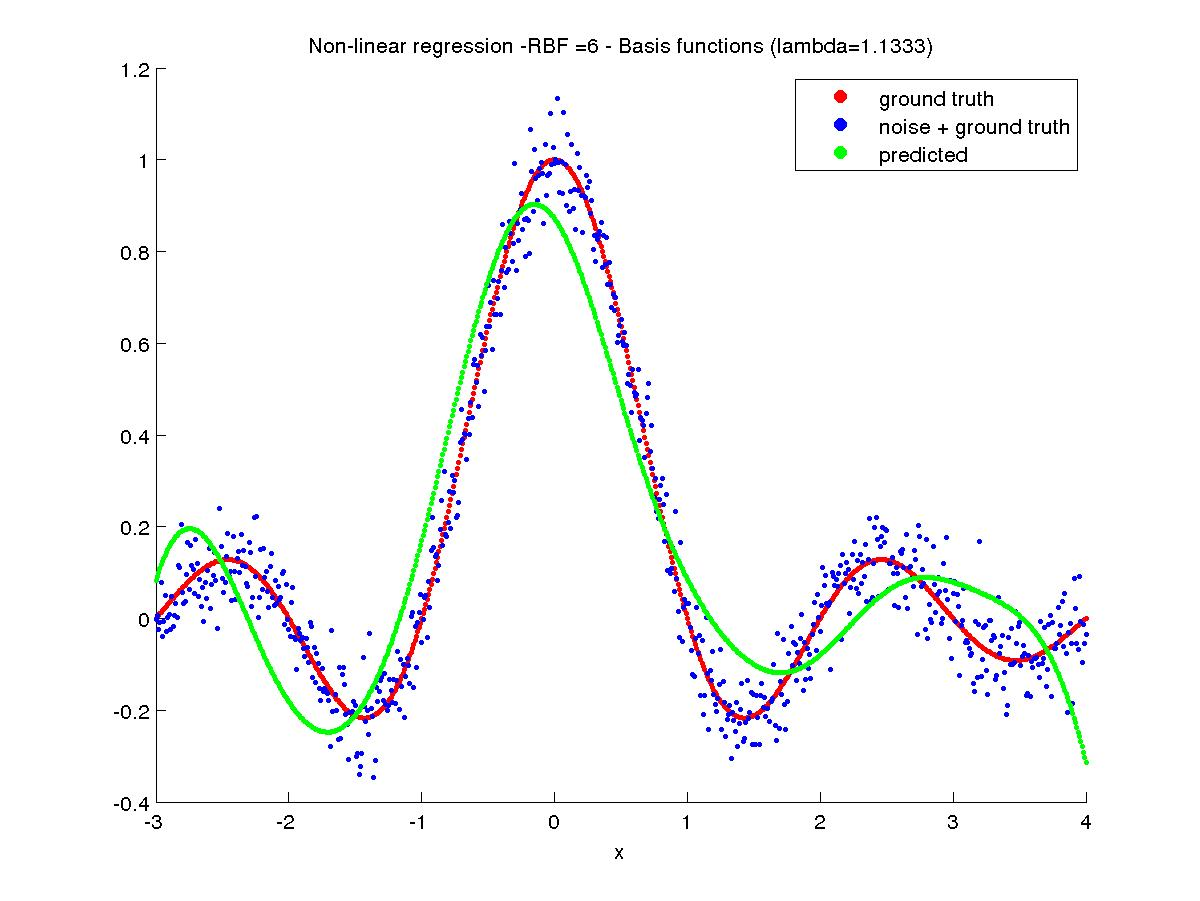
\includegraphics[scale=0.3]{./pics/task4/RBF =6 - Basis functions (lambda=1.1333)_train.jpg}

\subsubsection{Error analysis}

As shown in the error curves, the optimal value of $\lambda$ is found to be 1.1333 and the optimal number of kernel functions is 8.\\
When the $\lambda$ increases, the models tend to underfit the data and hence the prediction error increases.\\\\
Also, when the number of kernel function increases, normally the model will result in overfitting. However, since the dataset contains less noise, the overfitting behavior is not affecting the models.

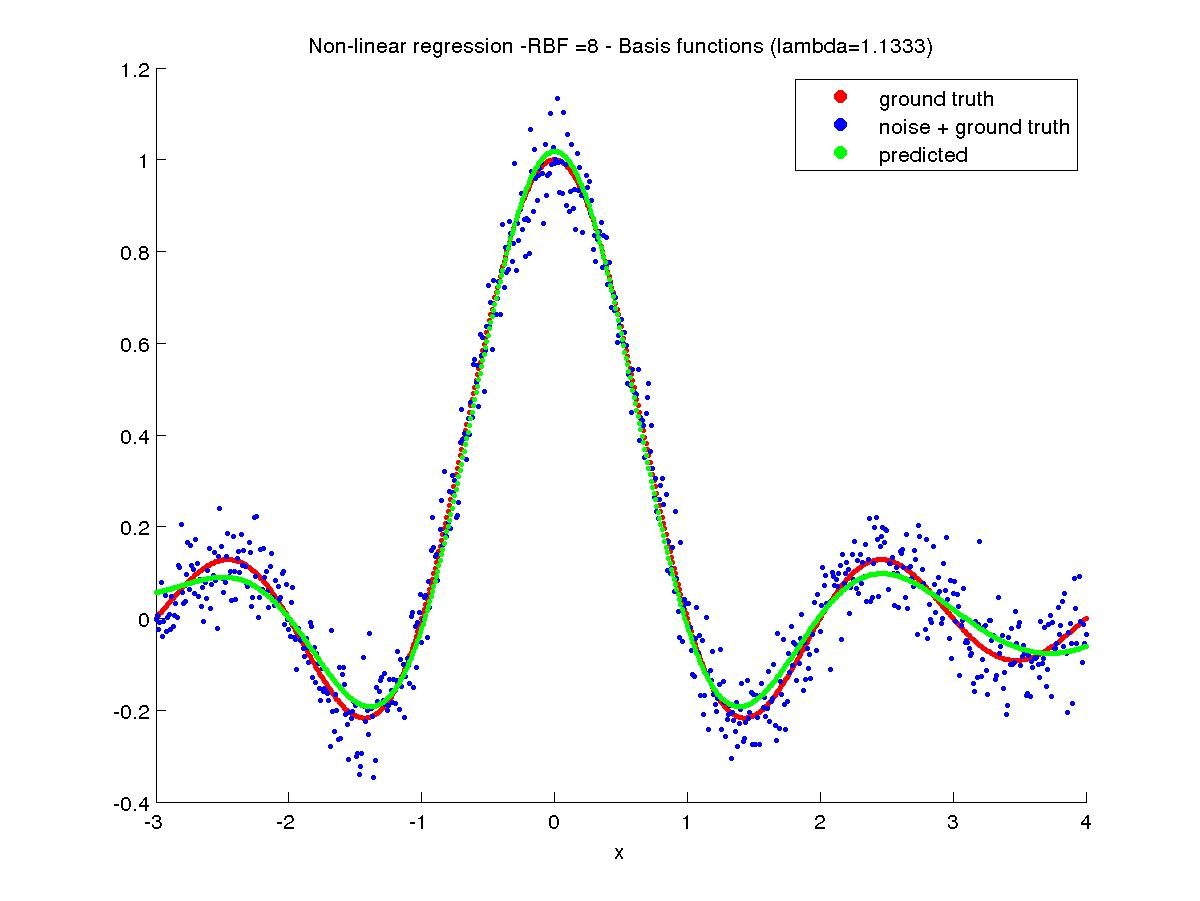
\includegraphics[scale=0.3]{./pics/task4/RBF =8 - Basis functions (lambda=1.1333)_train.jpg}

\begin{center}
  \begin{longtable}{ c | c }
	\multicolumn{1}{c}{$\lambda$ vs. Error} & 
	\multicolumn{1}{c}{Number of Kernel functions vs. Error}  \\
    \hline
    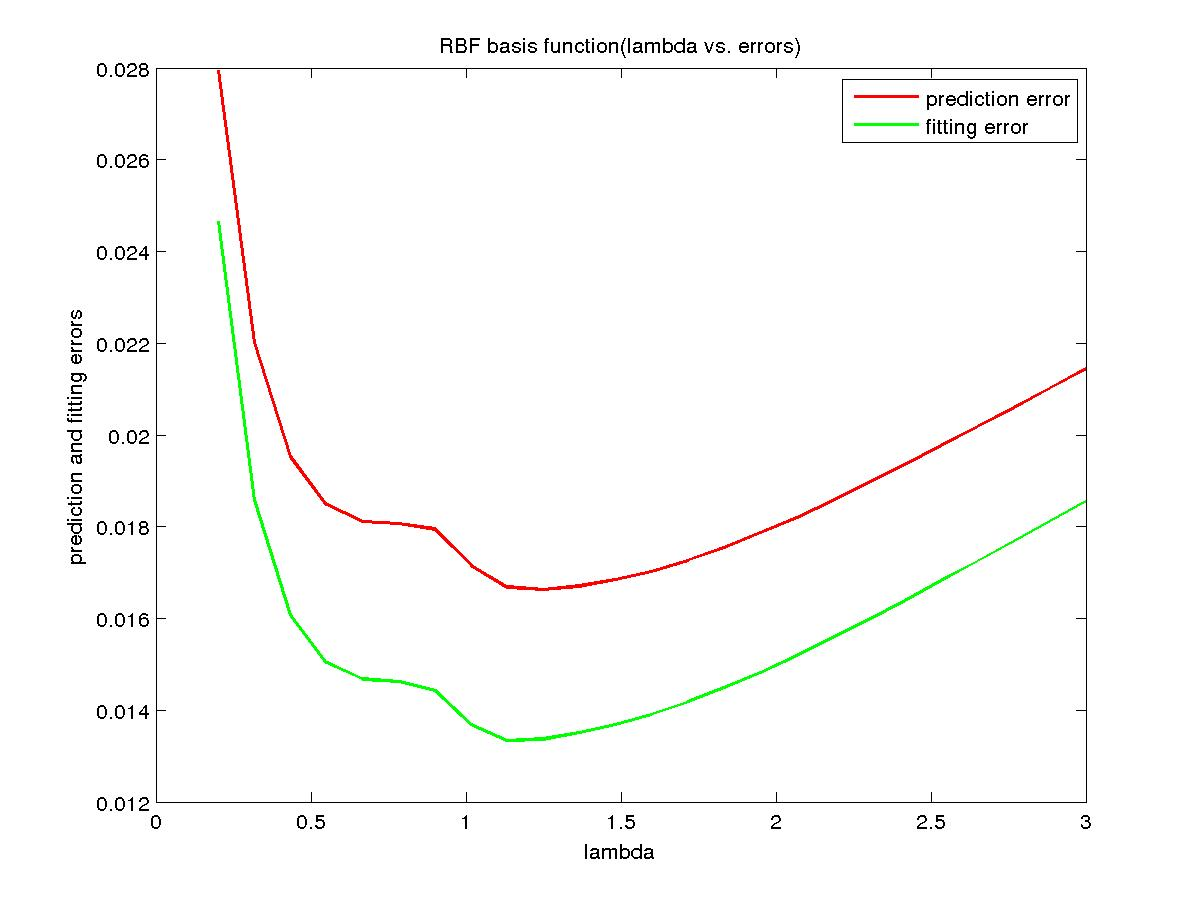
\includegraphics[scale=0.2]{./pics/task4/RBF basis function_fitting_lambda_errors.jpg}  & \includegraphics[scale=0.2]{./pics/task4/RBF basis function_numfunctions_errors.jpg} \\
    \hline
  \end{longtable}
\end{center}

\subsection{ARCTAN with 7 basis functions}

With 7 arc tangent functions, the predicted curve is given below: (prediction MSE = 0.0016)

\includegraphics[scale=0.3]{./pics/task4/arctan =7 - Basis functions(lambda=1.6)_train.jpg}

\subsubsection{Error analysis}
As shown in the error curves, the optimal value of $\lambda$ is found to be 1.6 and the optimal number of kernel functions is 10.

\includegraphics[scale=0.3]{./pics/task4/arctan =10 - Basis functions(lambda=1.6)_train.jpg}

\begin{center}
  \begin{longtable}{ c | c }
	\multicolumn{1}{c}{$\lambda$ vs. Error} & 
	\multicolumn{1}{c}{Number of Kernel functions vs. Error}  \\
    \hline
    \includegraphics[scale=0.2]{./pics/task4/ARCTAN basis function_fitting_lambda_errors.jpg}  & \includegraphics[scale=0.2]{./pics/task4/ARCTAN basis function_numfunctions_errors.jpg} \\
    \hline
  \end{longtable}
\end{center}

\newpage
\section{Relevance vector regression}

\subsection{$\lambda$ vs. MSE analysis}

\begin{center}
  \begin{longtable}{ c | c }
	\multicolumn{1}{c}{Train and Test errors for $\lambda$} & 
	\multicolumn{1}{c}{Training data model fit}  \\
    \hline
    \includegraphics[scale=0.4]{./pics/task5/rvr_train and test error.png}  & \includegraphics[scale=0.4]{./pics/task5/rvc_predicted_lambda=0.25007.png} \\
    \hline
  \end{longtable}
\end{center}

From the error plots for $\lambda$, the optimal $\lambda$ value is found to be 0.25007.\\

\begin{center}
  \begin{longtable}{ c | c }
	\multicolumn{1}{c}{Test data model fit} & 
	\multicolumn{1}{c}{Relevance vector weightage}  \\
    \hline
    \includegraphics[scale=0.4]{./pics/task5/rvc_test_predicted_lambda=0.25007.png}  & \includegraphics[scale=0.4]{./pics/task5/rvc_weights_lambda=0.25007.png} \\
    \hline
  \end{longtable}
\end{center}

\subsection{Non-linear regression to simulate Relevance vector regression}

Average MSE = 0.0015\\\\
\includegraphics[scale=0.4]{./pics/task5/non-linear-regression- rvr-random-1.png}
\includegraphics[scale=0.4]{./pics/task5/non-linear-regression- rvr-random-2.png}
\includegraphics[scale=0.4]{./pics/task5/non-linear-regression- rvr-random-3.png}
\includegraphics[scale=0.4]{./pics/task5/non-linear-regression- rvr-random-4.png}
\includegraphics[scale=0.4]{./pics/task5/non-linear-regression- rvr-random-5.png}

\end{document}